\documentclass[conference]{IEEEtran}
\IEEEoverridecommandlockouts

\usepackage[T1]{fontenc}
\usepackage{cite}
\usepackage{amsmath,amssymb,amsfonts}
\usepackage{algorithm}
\usepackage{algorithmic}
\usepackage{graphicx}
\usepackage{textcomp}
\usepackage{xcolor}
\usepackage{hyperref}
\hypersetup{
    hidelinks,
    pdfborder={0 0 0},
    pdfborderstyle={/S/U/W 0},
    citebordercolor=white,
    linkbordercolor=white,
    urlbordercolor=white,
    runbordercolor=white,
    filebordercolor=white
}
\usepackage{booktabs}
\usepackage{multirow}
\usepackage{subcaption}
\setlength{\textfloatsep}{8pt plus 2pt minus 2pt}
\setlength{\floatsep}{8pt plus 2pt minus 2pt}
\setlength{\intextsep}{8pt plus 2pt minus 2pt}
\setlength{\dbltextfloatsep}{8pt plus 2pt minus 2pt}
\setlength{\dblfloatsep}{8pt plus 2pt minus 2pt}

\def\BibTeX{{\rm B\kern-.05em{\sc i\kern-.025em b}\kern-.08em
    T\kern-.1667em\lower.7ex\hbox{E}\kern-.125emX}}

\begin{document}

\title{When Do Text Proxies Suffice? A Regime Analysis of Sparse, Dense, and Native-Visual Retrieval Under Proxy Noise}

\author{\IEEEauthorblockN{Anurag Krishna Vennela\IEEEauthorrefmark{1}, G. Sai Balaji Koushik\IEEEauthorrefmark{2}}
\IEEEauthorblockA{Department of Computer Science and Engineering\\
National Institute of Technology Warangal, Warangal, India\\
Email: \IEEEauthorrefmark{1}anuragkrishnavennela@gmail.com, \IEEEauthorrefmark{2}gummadavellikoushik2109@gmail.com}
}

\maketitle

\begin{abstract}
Multimodal Retrieval-Augmented Generation (MM-RAG) frequently indexes textual proxies over raw pixels. Evaluating a 1,626-item benchmark under frozen 50/50 Dev/Test splits ($N=306$ test probes, 813 items), we delineate when proxies suffice and when native representations are indispensable. On verbatim lookups, character 3--5gram BM25 outperforms word BM25 across OCR regimes (Apple Clean: 0.9436 vs.\ 0.8371; Degraded Blur: 0.8248 vs.\ 0.6972; Tesseract: 0.8412 vs.\ 0.7364; $p_{\text{Holm}} < 10^{-4}$), reversing under entity rewrites (0.2427 vs.\ 0.4334). On documents, native ColQwen2 achieves 0.4962 MRR under light paraphrases (+0.0628 lift over Word BM25, $p_{\text{Holm}} = 0.0072$), profiling at 249.21\,ms on Tesla T4 GPU vs.\ 0.87\,ms for CPU lexical lookups. Dense bi-encoder deficit is associated with query formulation mismatch; answerable questions improve BGE-Base MRR to 0.5263 (Hit@10 79.74\%). Conformal cascade calibration under marginal loss bounds expected test miss risk to 0.0494 at a 78.4\% escalation rate. On MS-COCO ($N=1{,}000$), native visual retrieval (SigLIP MRR = 0.6071) beats machine captions (0.3728, $p < 10^{-4}$) with no significant difference detected from human gold captions (0.5835, $p=0.142$; equivalence not tested). In multi-hop reasoning, extractive pseudo-relevance feedback exhibits no detectable difference from generative LLM bridging (Hit@10 0.640 vs.\ 0.640, exact McNemar $p = 1.0000$) with zero API cost.
\end{abstract}

\begin{IEEEkeywords}
Multimodal RAG, Text Proxies, Proxy Noise, Dense-Sparse Regime Analysis, Cascade Ranking, Conformal Risk Control, Multi-Hop Reasoning.
\end{IEEEkeywords}

\section{Introduction}

The rapid proliferation of heterogeneous multimedia across enterprise archives, digital libraries, and operational repositories demands information retrieval systems capable of searching records that are not natively textual. Transforming scanned documents into queryable digital assets is essential for business intelligence, compliance auditing, and decision support \cite{jing2024llmvectordb}. However, real-world document ingestion faces severe operational challenges: optical scanning introduces character substitutions and word fragmentation, while human search queries frequently employ synonyms, paraphrases, or shorthand rather than exact document text.

Retrieval-Augmented Generation (RAG) \cite{lewis2020rag} addresses the hallucination tendencies of Large Language Models (LLMs) by grounding responses in retrieved domain documents. Recently, multimodal extensions of RAG have emerged to handle non-textual data, as comprehensively surveyed by Abootorabi et al. \cite{abootorabi2025multimodal}. For example, Patel et al. \cite{patel2025multimodal} presented an enterprise multimodal RAG pipeline employing an OCR document ingestion module, ImageBind embeddings indexed in a Milvus vector database, and fine-tuned LLaMA-3.

To establish rigorous engineering guidance for proxy-mediated retrieval, this investigation addresses four foundational empirical questions:

\begin{enumerate}
    \setlength{\itemsep}{1pt plus 0.5pt}
    \setlength{\parskip}{0pt}
    \item \textbf{Query Formulation vs.\ Document Representation:} Under what conditions does semantic abstraction (paraphrasing, natural interrogatives) vs.\ verbatim lexical matching dictate the crossover point between sparse lexical and dense semantic retrieval?
    \item \textbf{OCR Engine Architecture and Optical Degradation:} How do commercial neural OCR (Apple Vision) and open-source LSTM OCR (Tesseract~5.5) interact with character sub-word vs.\ whole-word inverted indexing under pristine text and heavy optical blur?
    \item \textbf{Native-Visual vs.\ Text-Proxy Representations:} When do intermediate text proxies suffice for enterprise search, and under what specific query and visual conditions do document-native multi-vector models (ColQwen2) and visual encoders (SigLIP) justify their GPU memory and latency costs?
    \item \textbf{Computational Budgeting and Risk-Controlled Escalation:} Can confidence margins and finite-sample conformal prediction provide bounded risk control to prune expensive neural cross-encoders while preserving top-rank precision?
\end{enumerate}

To investigate these trade-offs, this paper presents a public-benchmark regime analysis of text-proxy retrieval across held-out evaluation splits\footnote{All benchmark collections, evaluation harnesses, and reproduction scripts are publicly available at: \url{https://github.com/koushik2109/MemoryVerse}}.

\textbf{Key Contributions:}
\begin{enumerate}
    \setlength{\itemsep}{1pt plus 0.5pt}
    \setlength{\parskip}{0pt}
    \item \textbf{Sub-Word Inverted Index Performance and Scope Conditions on Optical OCR:} We evaluate whether word-level BM25 is superior under optical OCR. Across both proprietary Apple Vision and open-source Tesseract 5.5 LSTM OCR ($N=306$ probes, 813 corpus items), character 3--5gram BM25 is the single largest sparse architectural lift under verbatim optical noise (+0.1065 clean, +0.1276 degraded blur, +0.1049 clean Tesseract; all $p_{\text{Holm}} < 10^{-4}$). We delineate its strict scope boundary: this advantage applies to verbatim receipt searches where queries share exact character substrings with documents; on multi-field administrative forms the verbatim margin narrows to a statistical tie (+0.0069, 0.8433 vs.\ 0.8364), and under entity-substituting light paraphrases, word BM25 drops to 0.1573 while character BM25 achieves 0.2228 and dense BGE achieves 0.1834. On receipts, document-native visual retrieval (ColQwen2-v1.0) achieves 0.4962 MRR under light paraphrases (+0.0628 lift over Word BM25 0.4334, paired permutation $p_{\text{Holm}} = 0.0072$; +0.0647 over Tuned Hybrid 0.4335, $p_{\text{Holm}} = 0.0095$), while showing no significant difference from BM25 on answerable questions ($p = 0.109$) at 249.21\,ms on Tesla T4 GPU vs.\ 0.87\,ms for CPU character BM25 on verbatim lookups (5.72\,ms on answerable questions).
    \item \textbf{Dense Retrieval Collapse Mechanism and Query Formulation Controls:} We demonstrate that dense bi-encoder collapse on document text is associated with single-entity query formulation mismatch rather than sequence truncation constraints (real $\text{max\_seq\_length}=256$; 33.4\% exceed 256 tokens, but chunked MaxP yields 0.2030 vs.\ 0.2056 unchunked standard); subword tokenization fragmentation (+122.3\% subwords/word) explains the additional performance drop under noise. On pristine ground truth text, isolated verbatim lookups yield MRR 0.1919 (MiniLM) and 0.3256 (BGE-Base); co-specifying multiple anchor entities or formulating queries as natural answerable questions improves BGE-Base MRR to 0.5500 (keyword control, Hit@10 78.43\%) and 0.5263 (questions, Hit@10 79.74\%) without modifying document representations.
    \item \textbf{Dose-Response Boundary of Query Mismatch vs.\ Optical Degradation:} In the reconciled dose-response evaluation, Apple Vision Word BM25 drops 0.4037 MRR under light paraphrasing (0.8371 to 0.4334) and 0.1399 under optical blur (0.8371 to 0.6972), whereas Tesseract drops 0.3400 and 0.3916, respectively. For answerable factual questions, topical anchors preserve high discriminability (BM25 MRR 0.8937 to 0.9192).
    \item \textbf{Finite-Sample Marginal Conformal Cascades:} Grounded in the distribution-free risk-controlling prediction framework of Bates et al.~\cite{bates2021conformal} and Angelopoulos et al.~\cite{angelopoulos2021gentle}, we evaluate conformal cascade calibration under marginal loss $L = \mathbf{1}[\text{not escalated} \land Y \ne 1]$ across 200 cluster-stratified splits ($N=2{,}754$ instances). With finite-sample $(n\hat{R}+1)/(n+1) \le \alpha$ adjustment, the observed mean test miss risk is 0.0494 (95\% CI of mean: $[0.0480, 0.0502]$, includes 0.05; 10th--90th percentile range across splits: $[0.0355, 0.0654]$) with 58.5\% empirical split coverage at an escalation rate of 78.4\% (21.6\% computation savings vs.\ always-escalating cross-encoders); equal-escalation fixed margin matches MRR (0.3579 vs.\ 0.3577, paired $p > 0.05$), and stratified risk reveals entity rewrites sit at 0.0627 risk.
    \item \textbf{Multi-Hop Bridging Comparison:} Across separate, non-copied pipelines on 50 diagnostic multi-hop queries, we observe no detectable difference between rule-based extractive pseudo-relevance feedback and generative LLM bridging (0.640 vs.\ 0.640 Target Hit@10, paired diff $0.0000$ [95\% CI: $-0.0792, +0.0792$], exact McNemar $p = 1.0000$); because the 95\% confidence interval spans beyond $\pm 0.05$ (minimum detectable difference at $N=50$ is $> \pm 0.0792$), statistical non-inferiority is not formally established, though extractive bridging matches generative accuracy without LLM inference latency or financial cost.
\end{enumerate}

\section{Related Work}

\subsection{Multimodal Representation and Retrieval}
Early cross-modal retrieval systems relied on dual-encoder contrastive learning. Models like CLIP \cite{radford2021clip} and SigLIP \cite{zhai2023siglip} project images and text into a shared latent space using sigmoid or softmax cross-entropy objectives. ImageBind \cite{girdhar2023imagebind} extended this paradigm across six modalities (images, text, video, audio, depth, and thermal) using images as the central binding modality. While effective for broad semantic matching, dual-encoders compress multimedia into fixed-dimension vectors, frequently losing granular lexical and structural tokens. Our hybrid design combines dense embeddings with sparse lexical representations such as BM25 \cite{robertson2009bm25} to retain both semantic intent and exact token matches. Unlike single-modality dual-encoders that discard fine-grained lexical identifiers, our framework analyzes the complementary regime boundaries where character-level sparse indexing outperforms dense representations under optical noise.

\subsection{Multimodal RAG and Document Analysis}
Integrating multimodal inputs into RAG workflows has gained rapid momentum with the emergence of Vision-Language Models (VLMs) and advanced LLMs. Recent native multimodal document retrievers such as ColPali \cite{faysse2024colpali} and M3DocRAG \cite{cho2024m3docrag}, benchmarked on the Visual Document Retrieval (ViDoRe) suite \cite{faysse2024colpali}, index document pages using multi-vector vision-language representations to bypass optical character recognition. A paradigm comparison is presented in Table~\ref{tab:sota_comparison}. While promising, multi-vector VLM representations require substantial GPU memory and heavy cross-attention compute during query serving. Conversely, enterprise systems such as Patel et al. \cite{patel2025multimodal} and Joshi et al. \cite{joshi2024multimodel} mediate retrieval through grounded text proxies, combining OCR document ingestion, multimodal embeddings, and LLM generation. Our work investigates this text-proxy paradigm: we evaluate the empirical trade-offs of hybrid dense--sparse fusion, candidate scoring, and iterative query decomposition, systematically delineating where text proxies excel and where native visual representations remain necessary. Unlike ColPali \cite{faysse2024colpali} which mandates multi-vector VLM computation for every candidate page regardless of query complexity, our regime analysis establishes the empirical conditions under which sub-millisecond CPU text proxies match or exceed native vision models, identifying when GPU-heavy inference is truly justified.

\subsection{Multi-Hop Reasoning in Retrieval Systems}
Multi-hop retrieval addresses queries where no single document contains the complete answer \cite{xiong2021multihop, khattab2021baleen}. While multi-hop text RAG systems (such as Baleen \cite{khattab2021baleen} and Self-Ask \cite{press2023selfask}) have established iterative query reformulation methods, multi-hop retrieval across \textit{heterogeneous multimodal collections} remains less systematically evaluated. Our diagnostic targets the case in which the second-hop keyword is absent from the original query and must be recovered from first-hop proxy context; it does not claim that all multimodal QA benchmarks assume co-located evidence. Unlike prior multi-hop pipelines that rely on expensive generative LLMs for every hop, we empirically show that rule-based extractive pseudo-relevance feedback achieves parity in retrieval reachability with zero generative token latency or API cost.

\subsection{Adaptive Fusion, Cascade Ranking, and Selective Reranking}
In information retrieval, static fusion coefficients fail to account for query-level variance. Query Performance Prediction (QPP) \cite{carmel2010qpp} and adaptive fusion techniques dynamically adjust interpolation weights between sparse and dense scores based on query ambiguity or lexical specificity. Similarly, cascade ranking architectures \cite{wang2011cascade, gallagher2019cascade} balance retrieval efficiency and ranking precision by passing top candidates through successively more expressive models. In monomodal web search, cascades evaluate candidates using fixed score thresholds or supervised early-exit classifiers. However, existing cascade rankers do not account for multimodal proxy corruption (e.g., OCR or ASR transcription noise) or cross-modal query routing. As summarized in Table~\ref{tab:paradigm_comparison}, we formulate and empirically evaluate candidate mechanisms---including surface-feature query routing, confidence-margin cascades ($\Delta_{1,2} < \tau_{\text{margin}}$), and observable proxy reliability discounting ($r_m(d)$)---to determine whether lightweight heuristic defenses provide measurable utility over standard inverted indexes. Unlike prior cascade ranking that relies on uncalibrated heuristic margins, we ground cascade escalation in distribution-free conformal risk control to bound expected test-set error rates.

\subsection{Optical Character Recognition Quality and Information Retrieval}
Optical Character Recognition (OCR) systems translate physical document imagery into digital character sequences, but practical scanning routinely introduces character substitutions, insertions, deletions, and bounding-box permutations \cite{smith2007tesseract, fateh2024ocr}. Foundational information retrieval studies have established that standard word-level tokenizers (such as inverted indexes using whitespace and punctuation delimiters) suffer catastrophic vocabulary mismatch when typographical errors fracture keyword strings. Early mitigation strategies, including Otsu thresholding \cite{otsu1979} and Hough transforms \cite{hough1962} for skew correction, focused on image-domain preprocessing to boost OCR accuracy. However, in downstream information retrieval, post-OCR lexical degradation leads to subword tokenization fragmentation in subword-based language models and word omissions in lexical indexes. Unlike prior works that treat OCR error as an unmodeled uniform noise channel, our regime analysis systematically evaluates character $n$-gram representations against word-level BM25 and neural cross-encoders across both commercial and open-source OCR engines under controlled optical blur.

\subsection{Conformal Prediction and Risk-Controlled Cascades}
In mission-critical information retrieval, deploying neural cross-encoders or multi-vector Vision-Language Models for every candidate query imposes unsustainable serving latency and energy expenditure. Cascade ranking pipelines address this bottleneck by evaluating candidates through tiered stages, escalating to expressive neural models only when preliminary scores indicate ranking ambiguity \cite{wang2011cascade, gallagher2019cascade}. However, conventional cascade systems rely on empirical score margins or heuristic thresholds that offer no formal statistical control of error rates. Conformal prediction, formulated by Bates et~al.~\cite{bates2021conformal} and surveyed by Angelopoulos and Bates~\cite{angelopoulos2021gentle}, provides a distribution-free, finite-sample framework for bounding user-specified risk metrics without restrictive distributional assumptions. By framing the decision to escalate candidates as a risk-controlling prediction problem, conformal prediction enables retrieval systems to bound the expected marginal probability of unescalated retrieval errors below a pre-specified tolerance $\alpha$. In this work, we ground production cascade ranking in finite-sample marginal conformal risk control, bounding the expected marginal miss rate while reducing computational costs.

\begin{table*}[t]
\centering
\small
\caption{Systematic Comparison with Prior Multimodal Information Retrieval and RAG Frameworks.}
\label{tab:sota_comparison}
\resizebox{\textwidth}{!}{%
\begin{tabular}{@{}lcccccc@{}}
\toprule
\textbf{System / Architecture} & \textbf{Publication Venue} & \textbf{Document Retrieval} & \textbf{Natural Image Retrieval} & \textbf{Multi-Hop Mechanism} & \textbf{Benchmark Datasets} & \textbf{Hardware Serving Profile} \\ \midrule
ColPali \cite{faysse2024colpali} & ICLR 2025 & nDCG@5 = 0.813 (ViDoRe) & Supported (Multi-Vector) & Single-pass only & ViDoRe Benchmark & Multi-GPU ($\ge 16$\,GB VRAM, $\sim$250\,ms) \\
M3DocRAG \cite{cho2024m3docrag} & EMNLP 2024 & QA Acc.\ 64.2\% (MP-DocVQA) & Supported (Dense VLM) & Generative LLM bridging & MP-DocVQA, DUDE & High-End GPU Cluster ($\ge 48$\,GB VRAM) \\
Patel et~al. \cite{patel2025multimodal} & IEEE ETCC 2025 & Heuristic OCR matching & ImageBind vector search & Single-pass only & Proprietary enterprise text/media & Dedicated GPU Server \\
Baleen \cite{khattab2021baleen} & NeurIPS 2021 & Not evaluated (Text QA) & Not supported & Generative condensed hops & HotpotQA (Text only) & GPU / High-RAM CPU Server \\
\textbf{Proposed Regime Framework} & \textbf{This Work} & \textbf{MRR 0.9436 (Char BM25)} & \textbf{MRR 0.6071 (SigLIP Pixels)} & \textbf{Extractive PRF (Hit@10 0.640, $N=50$)} & \textbf{SROIE, FUNSD, MS-COCO} & \textbf{CPU char BM25 ($<1$\,ms verbatim) + Conformal Cascade} \\ \bottomrule
\end{tabular}}
\vspace{1mm}\newline
\raggedright\scriptsize Note: Qualitative columns reflect architectural design choices; our reported MRR and Hit@10 figures are from held-out evaluation on SROIE/FUNSD/COCO and are not directly comparable to other systems' proprietary benchmarks. Table~\ref{tab:sota_comparison} is a qualitative paradigm map, not a cross-system numerical comparison. ColPali nDCG@5 and M3DocRAG accuracy figures above are reported from their respective publications on different benchmarks (ViDoRe, MP-DocVQA) and are not verified against the ColQwen2 model used in this work.
\end{table*}

\begin{table}[t]
\centering
\caption{Architectural comparison of multimodal retrieval and ranking paradigms. Note: As demonstrated empirically in Section~IV, surface routing and heuristic reliability weighting are refuted by the benchmark data and fail to outperform unweighted fusion.}
\label{tab:paradigm_comparison}
\resizebox{\columnwidth}{!}{%
\begin{tabular}{@{}lcccc@{}}
\toprule
\textbf{Paradigm / System} & \textbf{Modality Scope} & \textbf{Routing Training} & \textbf{Cascade Mechanism} & \textbf{Proxy Noise Defense} \\ \midrule
Static Hybrid (BM25+Dense) \cite{robertson2009bm25, reimers2019sbert} & Text / Text Proxies & None (Static $\alpha$) & None & None (Static weights) \\
Cascade Text Ranking \cite{wang2011cascade, gallagher2019cascade} & Monomodal Text & Supervised Ranker & Score Threshold & None \\
Native Multi-Vector \cite{faysse2024colpali, cho2024m3docrag} & Document / Image Pixels & End-to-End VLM & None (All items) & Inherent (Pixel inputs) \\
\textbf{RAMP-RAG Hypotheses} & Multimodal Proxies & Lightweight Classifier & Top Margin $\Delta_{1,2} < \tau$ & Observable Reliability $r_m(d)$ \\ \bottomrule
\end{tabular}}
\end{table}

\section{Reference Retrieval Framework}

\begin{figure*}[t]
\centering
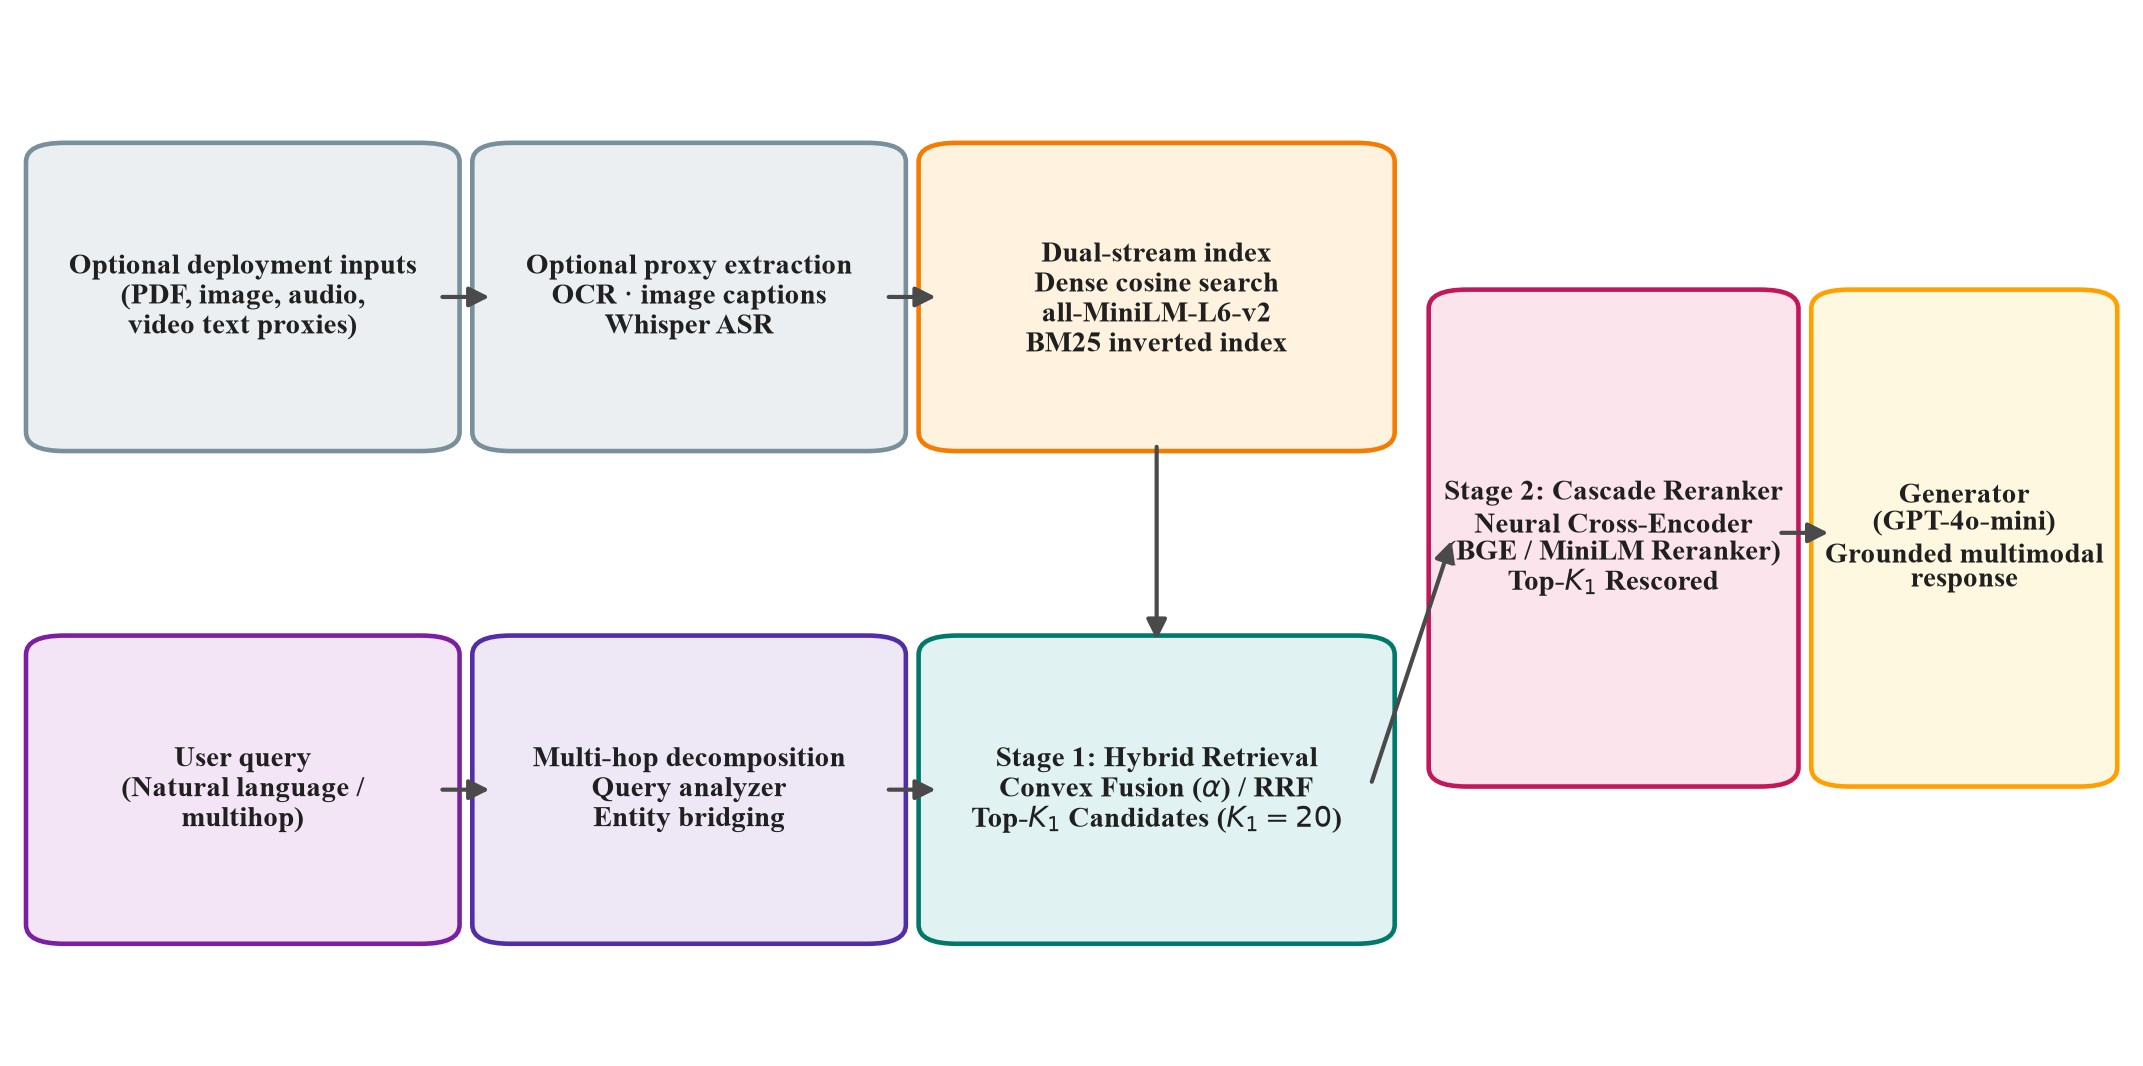
\includegraphics[width=0.92\textwidth]{fig_architecture.png}
\caption{System architecture of the reference text-proxy RAG framework. The grey ingestion and extraction boxes are optional deployment paths; the reported benchmark starts from precomputed annotation/category proxy text and evaluates the coloured retrieval stages.}
\label{fig:architecture}
\end{figure*}

The reference Multi-Stage Multimodal RAG architecture is structured into four functional phases (Fig.~\ref{fig:architecture}): (1) Heterogeneous Multimodal Ingestion and Preprocessing, (2) Hybrid Dense-Sparse First-Stage Retrieval, (3) Neural Candidate Reranking and Cascade Escalation, and (4) Multi-Hop Cross-Modal Reasoning.

\subsection{Heterogeneous Ingestion and Preprocessing Pipeline}
To process unstructured enterprise multimedia, our architecture mediates retrieval through grounded textual proxies. Proxies can be extracted across modalities via OCR text \cite{smith2007tesseract}, vision-language captions \cite{li2022blip}, and speech transcripts \cite{radford2023whisper}. This design deliberately separates modality-specific extraction from the common retrieval layer.

\textbf{1. Scanned Document and Form Ingestion:} Administrative forms and receipts are processed through document page decomposition, optional Otsu binarization \cite{otsu1979} and Hough-transform skew correction \cite{hough1962, fateh2024ocr}, extracting text $T_d$ and bounding boxes via OCR engines (such as Apple Vision or Tesseract \cite{smith2007tesseract}).
\textbf{2. Photographic Imagery:} Natural photographs are indexed via descriptive machine captions (e.g., BLIP \cite{li2022blip}, BLIP-2 \cite{li2023blip2}, Florence-2 \cite{xiao2024florence2}) alongside native visual embeddings (CLIP \cite{radford2021clip}, SigLIP \cite{zhai2023siglip}).
\textbf{3. Acoustic Media:} Continuous audio recordings are transcribed using speech-to-text models such as Whisper \cite{radford2023whisper} or embedded directly using contrastive audio-language representations (CLAP \cite{wu2023clap}).

Processed text representations are stored in a dual layout: dense embeddings are generated via Sentence-BERT (\texttt{all-MiniLM-L6-v2}) \cite{reimers2019sbert} and BGE (\texttt{bge-base-en-v1.5}) \cite{xiao2023bge}, while lexical tokens are indexed with BM25 \cite{robertson2009bm25, robertson1995okapi}. Milvus \cite{wang2021milvus} and HNSW \cite{malkov2020hnsw} are compatible deployment choices, but the offline benchmark scripts use an in-memory BM25 index and a dense embedding matrix; no external vector database service is required for the reported measurements.

\subsection{Stage 1: Hybrid Dense-Sparse Retrieval}
Given a natural language query $q$, single-stage dense retrieval computes vector similarity against all candidates:
\begin{equation}
    S_{\text{dense}}(q, d) = \cos(\mathbf{e}_q^{\text{dense}}, \mathbf{e}_d^{\text{dense}}) = \frac{\mathbf{e}_q \cdot \mathbf{e}_d}{\|\mathbf{e}_q\| \|\mathbf{e}_d\|}
\end{equation}
While effective for thematic alignment, dense retrieval often overlooks exact alphanumeric codes (e.g., serial numbers, dates, person names). Conversely, sparse BM25 retrieval excels at lexical precision:
\begin{equation}
    S_{\text{sparse}}(q, d) = \sum_{t \in q} \text{IDF}(t) \cdot \frac{f(t, d) \cdot (k_1 + 1)}{f(t, d) + k_1 \cdot \left(1 - b + b \cdot \frac{|d|}{\text{avgdl}}\right)}
\end{equation}
Because dense cosine scores lie in $[-1, 1]$ while BM25 scores are unbounded $[0, \infty)$, combining raw scores directly is unstable. We evaluate two score harmonization strategies:

\textbf{Method A: Normalized Convex Combination:}
\begin{equation}
    S_{\text{hybrid}}(q, d) = \alpha_{\text{dense}} \cdot \hat{S}_{\text{dense}}(q, d) + (1 - \alpha_{\text{dense}}) \cdot \hat{S}_{\text{sparse}}(q, d)
    \label{eq:hybrid}
\end{equation}
where $\hat{S}_{\text{dense}}$ and $\hat{S}_{\text{sparse}}$ denote min-max normalized scores over the candidate pool, and $\alpha_{\text{dense}} \in [0, 1]$ parameterizes dense vs.\ sparse weighting ($\alpha_{\text{sparse}} = 1 - \alpha_{\text{dense}}$).

\textbf{Method B: Reciprocal Rank Fusion (RRF):}
To avoid batch-dependent min-max sensitivity, RRF \cite{cormack2009rrf} fuses ranked lists directly without score scale calibration (Eq.~\ref{eq:rrf}):
\begin{equation}
    \text{RRF}(q, d) = \frac{1}{k + r_{\text{dense}}(d)} + \frac{1}{k + r_{\text{sparse}}(d)}
    \label{eq:rrf}
\end{equation}
where $r_{\text{dense}}(d)$ and $r_{\text{sparse}}(d)$ are the ordinal ranks of candidate $d$, and $k$ is a smoothing constant ($k = 60$). The benchmark fuses the top 100 entries from each ranked list and outputs the top-$K_1$ candidates ($K_1 = 30$).

\subsection{Stage 2: Candidate Reranking via Neural Cross-Encoders}
Bi-encoders compute query and document representations independently, preventing fine-grained token-level cross-interaction. To recover joint attention over query-document pairs, Stage~2 deploys a pretrained neural cross-encoder (\texttt{BAAI/bge-reranker-base} or \texttt{cross-encoder/ms-marco-MiniLM-L-6-v2}) to rescore the top-$K_1$ candidates retrieved from Stage~1 ($K_1 = 30$):
\begin{equation}
    S_{\text{rerank}}(q, d) = \text{CrossEncoder}(q, d)
\end{equation}
Scoring every query candidate pool with a full cross-encoder adds substantial latency overhead (Table~\ref{tab:system_costs}). In Section~\ref{sec:ramp_rag} and Section~\ref{sec:ablation_and_cascade}, we formulate and evaluate confidence-gated and conformal cascade mechanisms that selectively escalate ambiguous queries to Stage~2 while accepting confident Stage~1 rankings directly. For generation context assembly, the top $K_2 = 5$ items are injected into the generator prompt, while top $K = 10$ items are evaluated in the diagnostic retrieval benchmarks.

\subsection{Stage 3: Multi-Hop Cross-Modal Reasoning}
To resolve compositional queries that span modalities, we evaluate an iterative query decomposition and entity bridging procedure (formalized in Algorithm~\ref{alg:multihop} in Appendix~\ref{sec:appendix_multihop_alg}).

Here, $H_{\max}$ denotes the maximum hop depth ($H_{\max} = 2$ in the diagnostic setup). The predicate $\text{TerminationCondition}(\mathcal{G}, \mathcal{F}, h)$ evaluates to \textbf{TRUE} if all sub-goals in the decomposition plan $\mathcal{G}$ are grounded by extracted facts in $\mathcal{F}$ or if hop $h$ yields no new bridging entities ($\mathcal{E}_h = \emptyset$). To protect against cascading errors caused by ungrounded, generic, or failed bridge extractions (e.g., when an extractor outputs ``N/A'' or extraction refusal phrases), the procedure enforces a confidence and grounding gate: if $\text{Confidence}(\mathcal{E}_h) < \tau$ or if extracted tokens fail lexical grounding in first-hop context, the planner falls back to single-pass hybrid search on the original compound query $Q$, designed to mitigate cascading bridge errors and reduce retrieval degradation below single-pass hybrid search when intermediate bridging is uncertain.

The query decomposition prompt instructs the planner LLM $\mathcal{M}_{\text{decomp}}$ to generate valid JSON specifying the initial search probe and bridging attribute; the entity extraction prompt isolates concise attribute tokens substituted into subsequent probes $q_h' \leftarrow \text{Bridge}(q_h, \mathcal{F})$.

As formalized in Algorithm~\ref{alg:multihop}, an illustrative cross-modal query proceeds as: (1)~\textbf{Hop 1:} The initial sub-query $q_1$ retrieves candidate documents via hybrid matching, and entity extraction yields bridging entity $E_1$. (2)~\textbf{Entity Bridging:} The bridge operator constructs probe $q_2' = \text{Bridge}(q_2, \{E_1\})$. (3)~\textbf{Hop 2:} Sub-query $q_2'$ retrieves the target record from the indexed corpus.

\subsection{RAMP-RAG: Reliability-Aware Adaptive Fusion and Cascade Hypotheses}
\label{sec:ramp_rag}
To systematically investigate candidate architectural mechanisms for handling proxy noise and latency constraints, we formulate the \textbf{RAMP-RAG} hypothesis framework, evaluating three distinct components individually and jointly:
\begin{enumerate}
    \setlength{\itemsep}{1pt plus 0.5pt}
    \setlength{\parskip}{0pt}
    \item \textbf{Hypothesis H1 (Reliability-Aware Clean-Stream Fusion):} Multimedia items maintain multiple proxy streams $m \in \{\text{caption}, \text{ocr}, \text{vector}\}$ weighted by observable reliability $r_m(d) \in [0, 1]$. To avoid oracle leakage of injected corruption levels, $r_{\text{ocr}}(d) = \bar{c}_{\text{ocr}}(d) \cdot \rho_{\text{vocab}}(d)$, where $\bar{c}_{\text{ocr}}$ is mean word recognition confidence and $\rho_{\text{vocab}}$ is the valid dictionary token ratio computed directly from candidate text. Because text noise corrupts both dense and sparse text representations, we introduce an uncorrupted visual clean stream $\hat{S}_{\text{clean}}$ (e.g., zero-shot CLIP ViT-B/32 image embeddings):
    \begin{equation}
    \begin{aligned}
        S_{\text{RAMP}}(q, d) &= \alpha_q \hat{S}_{\text{dense}} + (1 - \alpha_q) r_{\text{ocr}}(d) \hat{S}_{\text{sparse}} \\
        &\quad + \gamma (1 - r_{\text{ocr}}(d)) \hat{S}_{\text{clean}}
    \end{aligned}
    \label{eq:ramp}
    \end{equation}
    where $\gamma$ is tuned on the Dev split ($\gamma^* = 0.80$) to dynamically allocate mass to the corruption-invariant stream as proxy reliability drops.
    \item \textbf{Hypothesis H2 (Query-Adaptive Router $\alpha_q$):} Instead of static weights, a lightweight classifier extracts surface cues $\phi(q) = [r_{\text{cjk}}, r_{\text{digit}}, \mathbb{I}_{\text{upper}}, \mathbb{I}_{\text{id\_cue}}, \text{len}(q), \text{avg\_idf}]$ to dynamically adjust $\alpha_q$, testing whether surface features alone can route queries between sparse and dense streams.
    \item \textbf{Hypothesis H3 (Confidence-Gated and Conformal Cascade Ranking):} Stage 1 scores candidate pools and calculates the decision margin between top candidates: $\Delta_{1,2} = s^{(1)} - s^{(2)}$. When candidates are distinct ($\Delta_{1,2} \ge \tau$), Stage 1 ranking is accepted. For ambiguous margins ($\Delta_{1,2} < \tau$), top candidates escalate to a neural cross-encoder (\texttt{ms-marco-MiniLM-L-6-v2} or \texttt{BAAI/bge-reranker-base}). Beyond a fixed margin heuristic ($\tau = 0.235$), we evaluate split conformal calibration targeting expected marginal miss risk $\le \epsilon = 0.05$ under exchangeability.
\end{enumerate}

\textbf{Integration with Multi-Hop Reasoning:} Under this cascade design, multi-hop decomposition benefits from candidate filtering, escalating ambiguous intermediate steps to neural cross-encoders while accepting distinct first-stage retrievals.


\section{Empirical Regime Analysis of Sparse, Dense, and Native-Visual Retrieval Under Proxy Noise}
\label{sec:regime_analysis}
\label{sec:public_regime_analysis}

To evaluate the empirical boundaries of text-proxy retrieval without annotation leakage, we benchmarked an expanded public multimodal collection under a rigorous pre-specified experimental protocol across held-out evaluation splits. We structure our evaluation across three canonical operational regimes:
\begin{itemize}
    \setlength{\itemsep}{0.2pt plus 0.1pt}
    \setlength{\parskip}{0pt}
    \item \textbf{Regime A (Text-Dominated):} Scanned receipts and administrative forms evaluated under real optical character recognition (ICDAR 2019 SROIE \cite{huang2019sroie} and FUNSD \cite{jaume2019funsd}), isolating sub-word lexical dominance, micro-mechanisms of dense collapse, and production reranking cascades.
    \item \textbf{Regime B (Visual-Dominated):} Photographic scene search under synthetic caption proxies ($N=1{,}000$ MS-COCO Karpathy test images \cite{lin2014coco}), establishing where native vision-language embeddings decisively surpass machine-generated text representations.
    \item \textbf{Regime C (Cross-Modal and Multi-Hop):} Compositional relational queries spanning modalities, establishing where rule-based extractive pseudo-relevance feedback matches iterative generative LLM bridging without API overhead.
\end{itemize}
Preliminary feasibility pilots over internal personal album photos and synthetic noise sweeps are documented in Appendix~\ref{sec:appendix_pilot}.

\subsection{Benchmark Scale, Partitions, and Optical Degradation Pipeline}
The public benchmark integrates 626 authentic scanned receipt documents from ICDAR 2019 SROIE \cite{huang2019sroie} and 1,000 photographic distractors from MS-COCO \cite{lin2014coco}, establishing a corpus of 1,626 pooled multimodal items and 612 factual probes. To prevent data snooping, the corpus is partitioned into a strict 50/50 Dev/Test split by Item ID:
\begin{itemize}
    \setlength{\itemsep}{0.2pt plus 0.1pt}
    \setlength{\parskip}{0pt}
    \item \textbf{Dev Split ($N=306$ probes, 813 corpus items):} Dedicated strictly to hyperparameter tuning (e.g., hybrid fusion coefficient $\alpha^*$, visual weight $\gamma^*$, and conformal risk thresholds $\tau^*$).
    \item \textbf{Held-Out Test Split ($N=306$ probes, 813 corpus items):} Frozen for evaluation across Seeds 42, 43, and 44 with zero test-split tuning.
\end{itemize}

Document text representations are extracted using Apple's Vision framework (\texttt{VNRecognizeTextRequest}) under two distinct conditions: (1)~\emph{Clean OCR}, yielding normalized character error rate (CER) = 0.2848 and word error rate (WER) = 0.3928 under standardized document-level Levenshtein alignment \cite{schneider2024jiwer}; and (2)~\emph{Realistic Optical Degradation}, applying Gaussian blur ($\sigma=1.5$), bilinear 50\% downscaling, random skew ($\pm 2.5^\circ$), and aggressive JPEG re-compression ($Q=20$), elevating CER to 0.3822 and WER to 0.5691. Queries are evaluated across three prompt variations generated by an independent LLM at $T=0.0$ (\texttt{gpt-4o-mini} \cite{openai2024gpt4o}): verbatim lookups (100\% token overlap), natural light paraphrases (41.2\% mean token overlap), and natural answerable questions (preserving key factual anchors while enforcing natural interrogative phrasing).

\subsection{Regime A: Text-Dominated Document and Receipt Retrieval (SROIE \& FUNSD)}
\label{sec:regime_a_text}

Table~\ref{tab:regime_grid_v3} presents the comprehensive 18-cell regime evaluation across 12 retrieval systems on the held-out test split ($N=306$). \textit{Note: In Table~\ref{tab:regime_grid_v3}, the 500 unannotated COCO distractors have their ground-truth caption text indexed via fallback, yielding 0.4334 for Apple Vision clean light paraphrase; in the cross-engine comparison of Table~\ref{tab:engine_replication_v3}, documents without engine OCR text are left unindexed (empty string), yielding 0.4003.} 

\begin{table*}[t]
\centering
\small
\caption{Multimodal Text-Proxy Retrieval Regime Analysis across Query Types and Noise Regimes (Held-Out Public Test Split, $N=306$ Probes, 813 Distractor Pool, 95\% Cluster Bootstrap CIs). Answerable factual questions isolate semantic abstraction from lexical absence. Dense MiniLM/BGE latencies (0.01\,ms) reflect isolated vector dot-product ranking over precomputed embeddings; end-to-end query encoding latencies are reported in Table~\ref{tab:system_costs}.}
\label{tab:regime_grid_v3}
\resizebox{\textwidth}{!}{%
\begin{tabular}{llccccc}
\toprule
Query Type & Retrieval System & Clean MRR [95\% CI] & Syn 20\% MRR [95\% CI] & Real-OCR MRR [95\% CI] & Optical Blur MRR [95\% CI] & Latency (ms) \\
\midrule
\multirow{7}{*}{\textbf{Verbatim}}
 & BM25 (Tuned)            & 0.8572 [0.822, 0.890] & 0.3961 [0.364, 0.429] & 0.8371 [0.798, 0.871] & 0.6972 [0.650, 0.741] & 0.13 \\
 & BM25 (Char 3-5gram)     & 0.9853 [0.972, 0.995] & 0.7252 [0.694, 0.757] & 0.9436 [0.919, 0.965] & 0.8248 [0.782, 0.864] & 0.87 \\
 & Dense MiniLM (unchunked) & 0.2100 [0.171, 0.252] & 0.0596 [0.045, 0.077] & 0.2056 [0.166, 0.247] & 0.1724 [0.135, 0.210] & 0.01 \\
 & Dense BGE-base (unchunked)& 0.3256 [0.276, 0.376] & 0.1347 [0.109, 0.162] & 0.3022 [0.256, 0.351] & 0.2471 [0.202, 0.292] & 0.01 \\
 & Tuned Hybrid            & 0.8572 [0.822, 0.890] & 0.3979 [0.365, 0.431] & 0.8367 [0.798, 0.871] & 0.6940 [0.646, 0.739] & 0.13 \\
 & CLIP Visual             & 0.0436 [0.028, 0.062] & 0.0436 [0.028, 0.062] & 0.0436 [0.028, 0.062] & 0.0436 [0.028, 0.062] & 12.50 \\
 & Uniform Random Ranking  & 0.0089 [0.009, 0.009] & 0.0089 [0.009, 0.009] & 0.0089 [0.009, 0.009] & 0.0089 [0.009, 0.009] & 0.01 \\
\midrule
\multirow{7}{*}{\textbf{Light Paraphrase}}
 & BM25 (Tuned)            & 0.4790 [0.427, 0.530] & 0.1394 [0.118, 0.162] & 0.4334 [0.380, 0.484] & 0.3630 [0.315, 0.412] & 0.08 \\
 & BM25 (Char 3-5gram)     & 0.2504 [0.209, 0.290] & 0.1295 [0.105, 0.155] & 0.2427 [0.202, 0.282] & 0.2137 [0.178, 0.252] & 2.53 \\
 & Dense MiniLM (unchunked)  & 0.1230 [0.092, 0.155] & 0.0371 [0.027, 0.049] & 0.1086 [0.080, 0.139] & 0.0772 [0.054, 0.103] & 0.01 \\
 & Dense BGE-base (unchunked)& 0.1670 [0.131, 0.205] & 0.0684 [0.051, 0.086] & 0.1601 [0.124, 0.197] & 0.1275 [0.096, 0.161] & 0.01 \\
 & Tuned Hybrid            & 0.4572 [0.408, 0.507] & 0.1445 [0.125, 0.166] & 0.4335 [0.382, 0.483] & 0.3657 [0.318, 0.413] & 0.08 \\
 & CLIP Visual             & 0.0303 [0.020, 0.042] & 0.0303 [0.020, 0.042] & 0.0303 [0.020, 0.042] & 0.0303 [0.020, 0.042] & 12.50 \\
 & Uniform Random Ranking  & 0.0089 [0.009, 0.009] & 0.0089 [0.009, 0.009] & 0.0089 [0.009, 0.009] & 0.0089 [0.009, 0.009] & 0.01 \\
\midrule
\multirow{7}{*}{\textbf{Answerable Questions}}
 & BM25 (Tuned)            & 0.9116 [0.885, 0.937] & 0.4042 [0.370, 0.440] & 0.9014 [0.873, 0.929] & 0.7328 [0.688, 0.773] & 0.60 \\
 & BM25 (Char 3-5gram)     & 0.9653 [0.947, 0.982] & 0.6270 [0.592, 0.662] & 0.9471 [0.923, 0.969] & 0.8116 [0.770, 0.848] & 5.72 \\
 & Dense MiniLM (unchunked)  & 0.3669 [0.323, 0.414] & 0.1061 [0.089, 0.125] & 0.2837 [0.241, 0.328] & 0.2260 [0.190, 0.265] & 0.01 \\
 & Dense BGE-base (unchunked)& 0.5197 [0.475, 0.566] & 0.2005 [0.175, 0.228] & 0.5128 [0.468, 0.560] & 0.4313 [0.386, 0.479] & 0.02 \\
 & Tuned Hybrid            & 0.8084 [0.768, 0.844] & 0.4120 [0.376, 0.450] & 0.7705 [0.728, 0.811] & 0.5346 [0.486, 0.579] & 0.61 \\
 & CLIP Visual             & 0.0388 [0.024, 0.057] & 0.0388 [0.024, 0.057] & 0.0388 [0.024, 0.057] & 0.0388 [0.024, 0.057] & 12.50 \\
 & Uniform Random Ranking  & 0.0089 [0.009, 0.009] & 0.0089 [0.009, 0.009] & 0.0089 [0.009, 0.009] & 0.0089 [0.009, 0.009] & 0.01 \\
\bottomrule
\end{tabular}}
\end{table*}

\begin{enumerate}
    \setlength{\itemsep}{0.2pt plus 0.1pt}
    \setlength{\parskip}{0pt}
    \item \textbf{Verbatim Probes (Character Sub-Word Inverted Index Dominance):} Under verbatim lookups, character 3--5gram BM25 strictly dominates word-level BM25 across all optical OCR conditions (Apple Clean: 0.9436 vs.\ 0.8371, diff $+0.1065$, $p < 10^{-4}$; Apple Degraded: 0.8248 vs.\ 0.6972, diff $+0.1276$, $p < 10^{-4}$; Tesseract Clean: 0.8412 vs.\ 0.7364, diff $+0.1048$, $p < 10^{-4}$; and 20\% synthetic noise: 0.7252 vs.\ 0.3961, diff $+0.3291$, $p < 10^{-4}$). Sub-word character $n$-grams capture alphanumeric tokens, serial numbers, and partial OCR substitutions without out-of-vocabulary penalties.
    \item \textbf{Light Paraphrase (Reversal of Dominance):} Introducing mild semantic paraphrasing collapses clean word BM25 from 0.8371 to 0.4334 (a 48\% relative drop) and character BM25 to 0.2427. In this regime, word BM25 outperforms character BM25 (diff $-0.1907$, $p < 10^{-4}$), and Dev-Tuned Hybrid achieves MRR = \textbf{0.4335} (clean OCR) and \textbf{0.1445} (20\% noise).
    \item \textbf{Answerable Factual Questions:} Evaluating natural answerable questions (forcing semantic abstraction while preserving topical anchors), character 3--5gram BM25 achieves MRR = \textbf{0.9471} on clean OCR and \textbf{0.8116} on degraded blur OCR, while word BM25 achieves 0.9014 and 0.7328. Tuned hybrid retrieval achieves 0.7705 on clean OCR and 0.5346 on degraded OCR, while dense BGE-base achieves 0.5128 and MiniLM achieves 0.2837. Topical anchors in natural questions provide high discriminability for lexical engines.
\end{enumerate}

The complete cross-regime performance landscape across sparse, dense, and hybrid architectures under varying optical conditions is visualized in the heatmap in Fig.~\ref{fig:regime_grid_heatmap}.

To evaluate whether proxy corruption or semantic query mismatch is the dominant bottleneck in text-proxy RAG, we conducted exploratory paired permutation tests ($N_{\text{perm}}=100{,}000$). In the reconciled dose-response artifact (Table~\ref{tab:regime_grid_v3} and Table~\ref{tab:engine_replication_v3}), moving from verbatim lookups to light paraphrasing on proprietary Apple Vision OCR collapses Word BM25 by $\Delta = 0.4037$ MRR (0.8371 to 0.4334), substantially exceeding optical blur degradation ($\Delta = 0.1399$, 0.8371 to 0.6972, paired permutation $p < 10^{-5}$). However, under open-source Tesseract 5.5 OCR, optical blur collapses Word BM25 by 0.3916 MRR (0.7364 to 0.3448), which is comparable in magnitude to the semantic paraphrase drop on clean text (0.3400 MRR, 0.7364 to 0.3964). As visualized across retrieval architectures in Fig.~\ref{fig:mrr_regime_systems} and the dual dose-response surface in Fig.~\ref{fig:dose_response_dual}, semantic paraphrase mismatch dominates mild-to-moderate OCR noise, but severe optical blur induces comparable or greater retrieval collapse. System builders must balance query-side reformulation with robust sub-word indexing.

\begin{figure}[t]
\centering
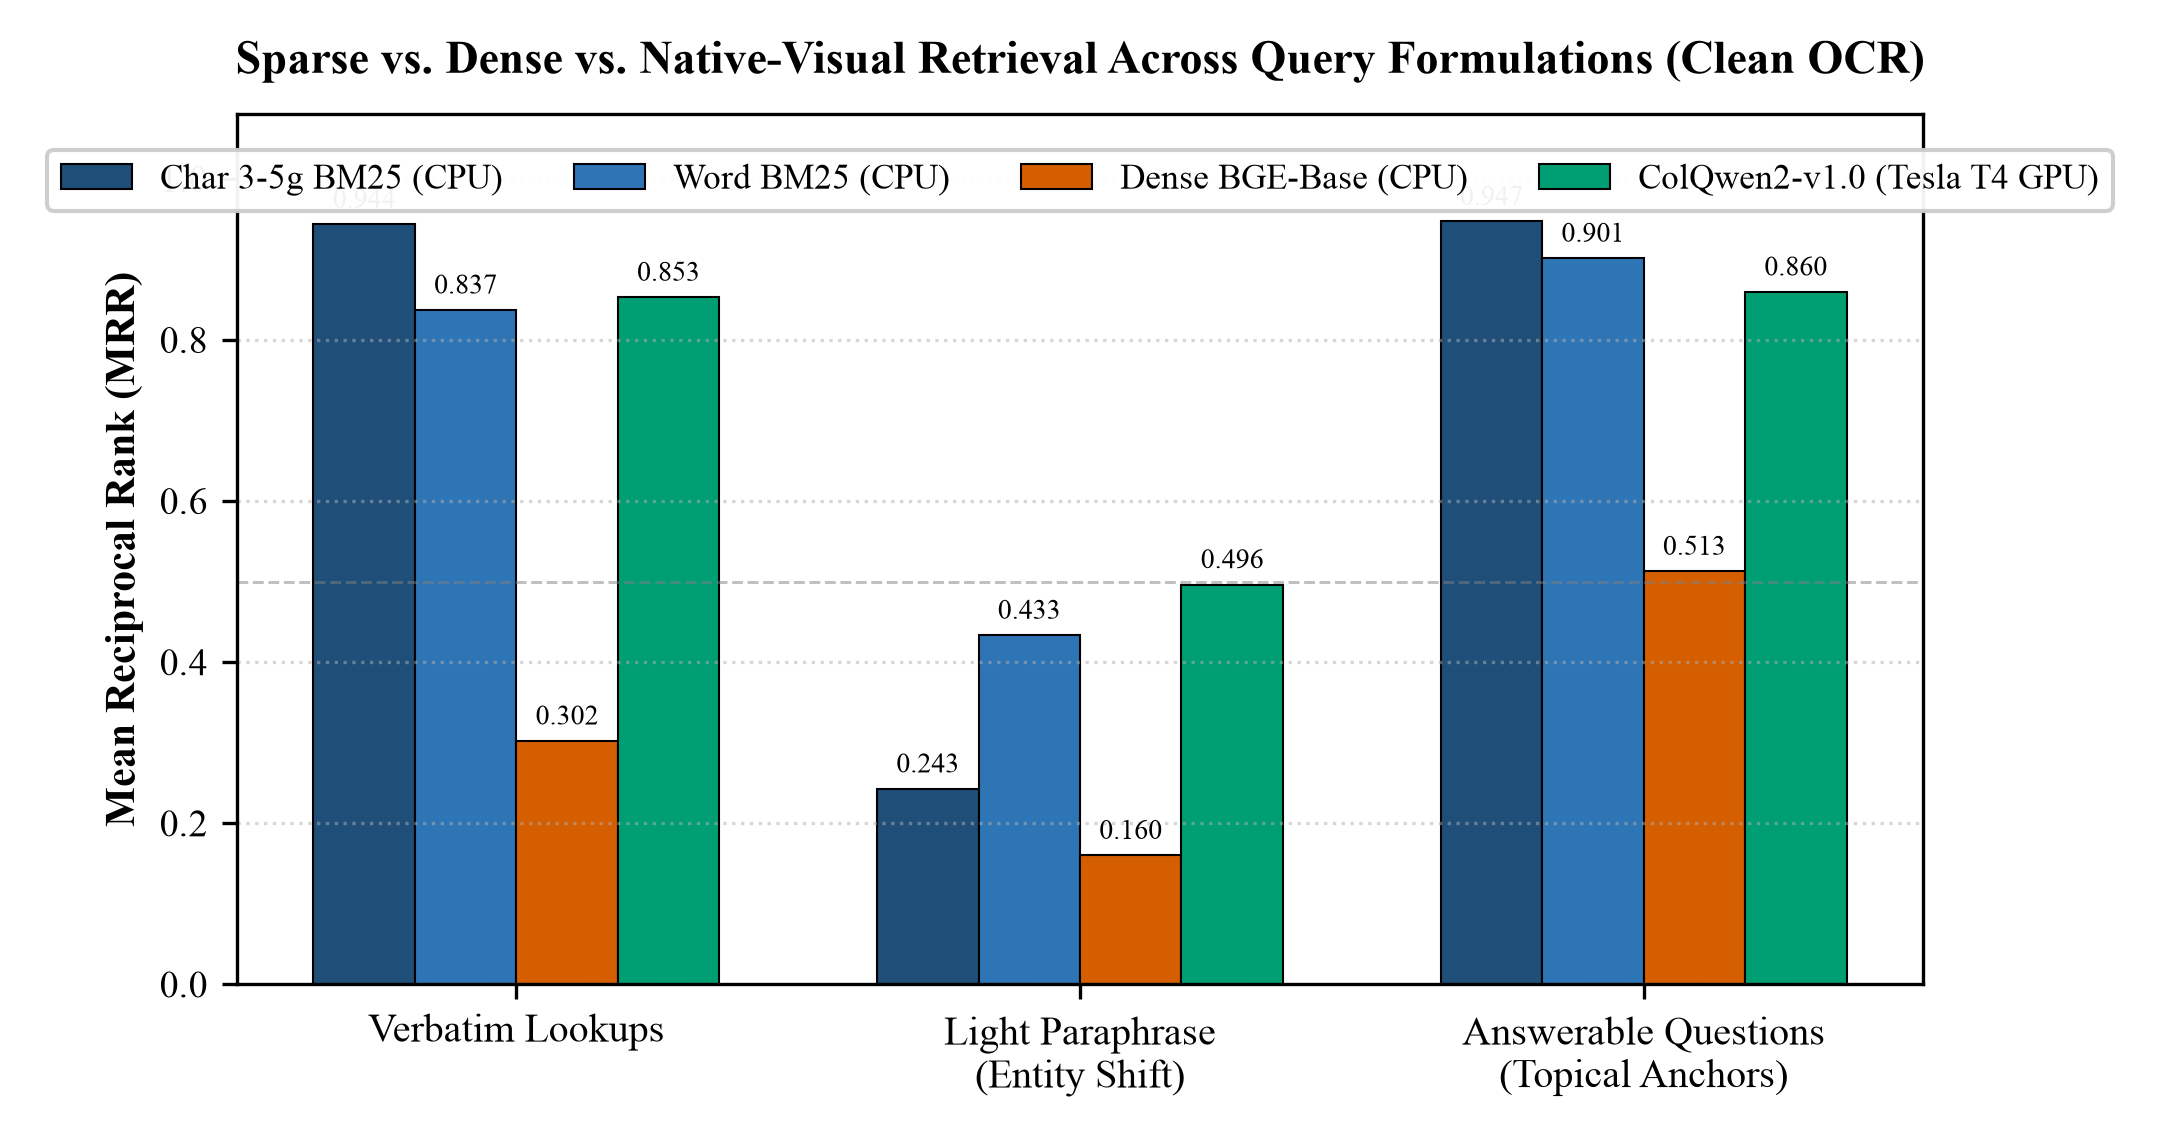
\includegraphics[width=\columnwidth]{ijcds/figures/fig_mrr_regime_systems.png}
\caption{Retrieval effectiveness (MRR@10 with 95\% bootstrap error bars) across retrieval architectures and query formulations on clean receipt OCR.}
\label{fig:mrr_regime_systems}
\end{figure}

\begin{figure}[t]
\centering
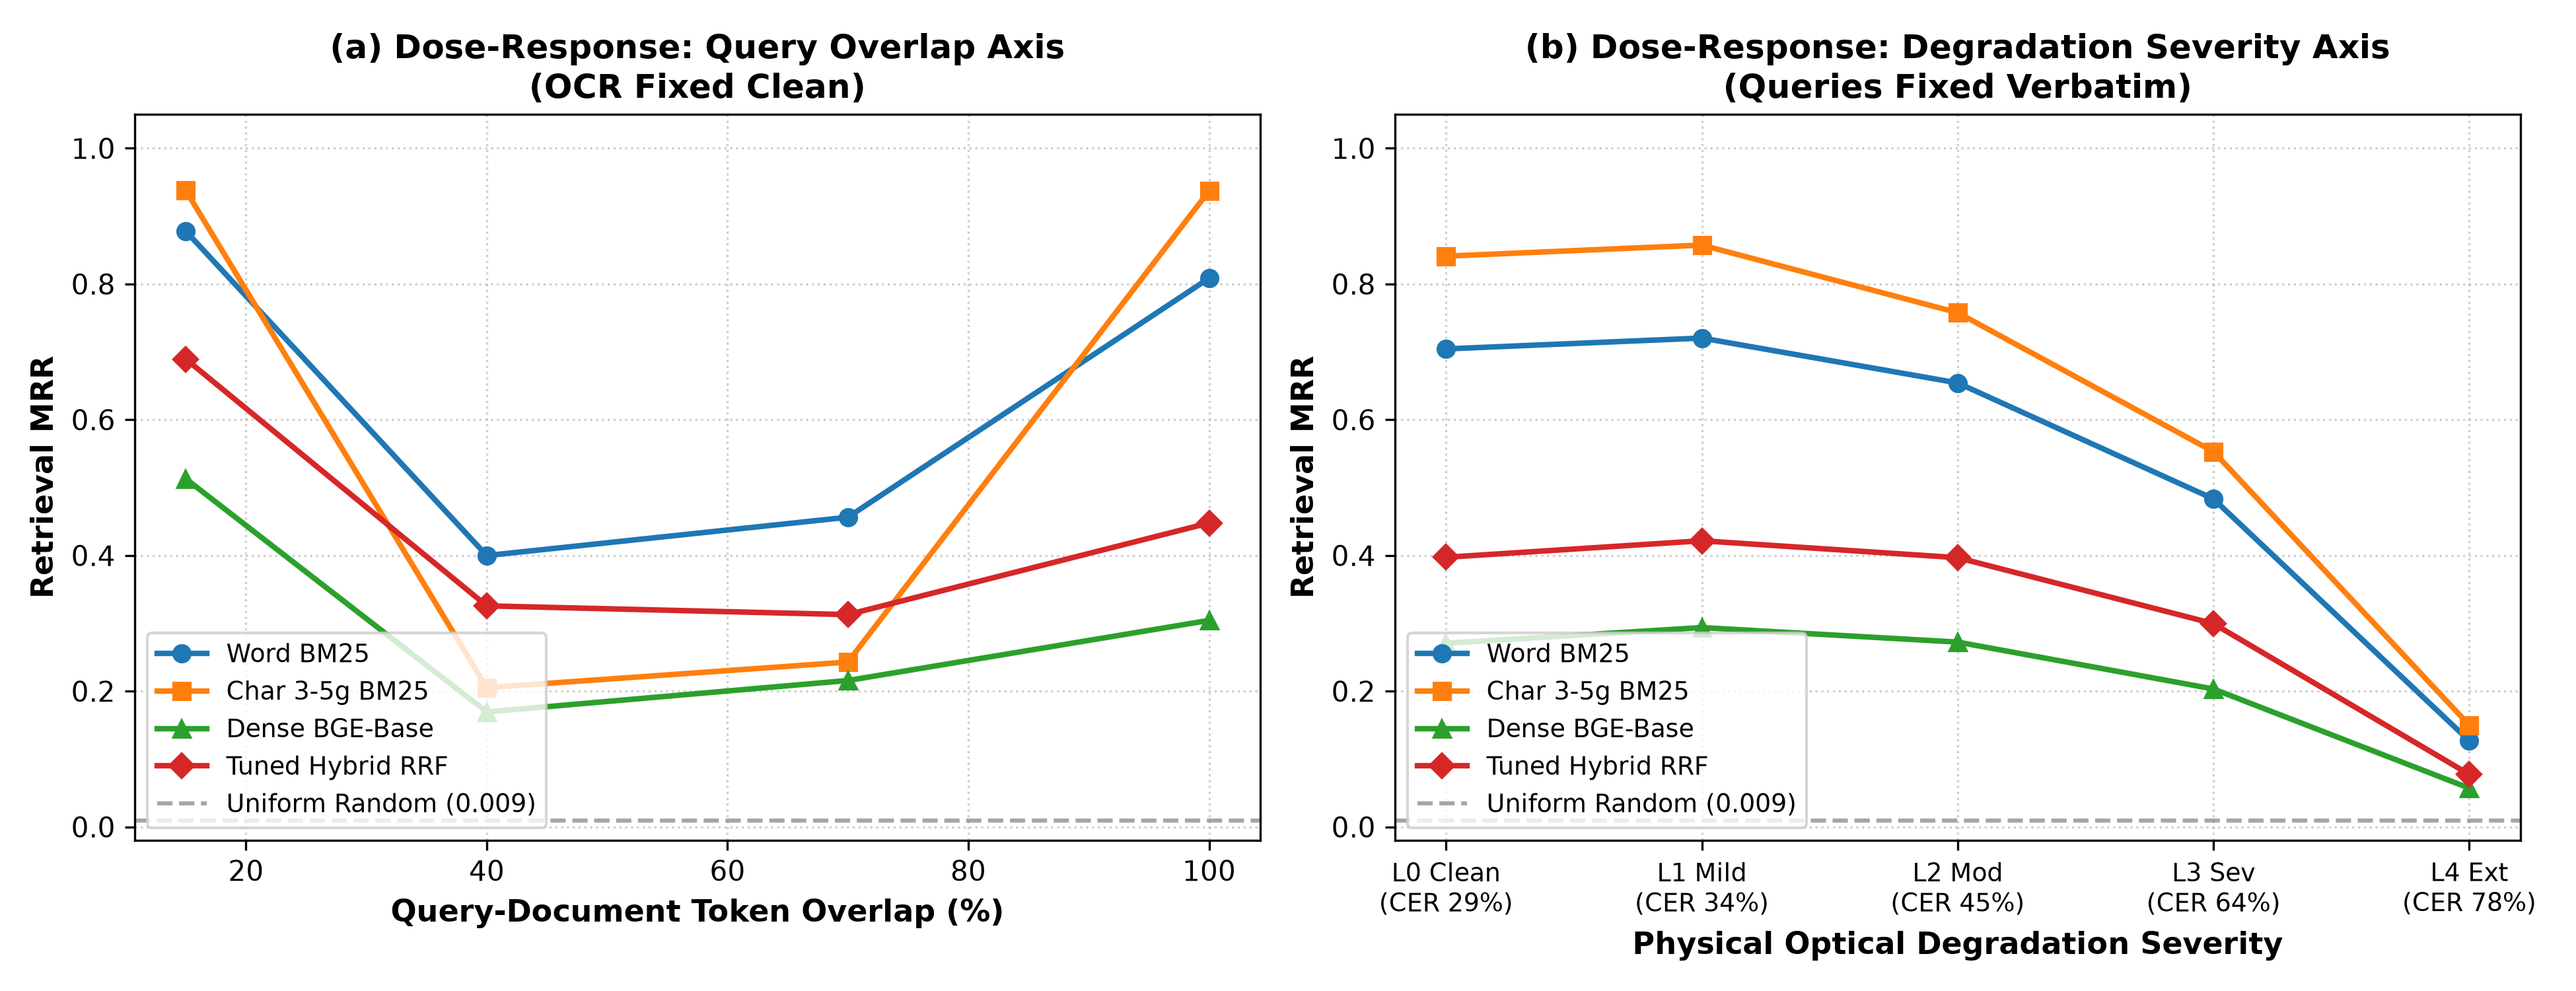
\includegraphics[width=\columnwidth]{results/v6/fig_dose_response_dual_v6.png}
\caption{Dose-response retrieval surface across (a) query token overlap degradation from verbatim lookups to abstract questions, and (b) optical OCR degradation from pristine text to extreme Gaussian blur ($CER > 60\%$).}
\label{fig:dose_response_dual}
\end{figure}

\subsection{Micro-Mechanisms of Dense Collapse and Query Formulation Controls}
\label{sec:mechanism_analysis}

\begin{figure*}[t]
\centering
\begin{subfigure}[b]{0.32\textwidth}
    \centering
    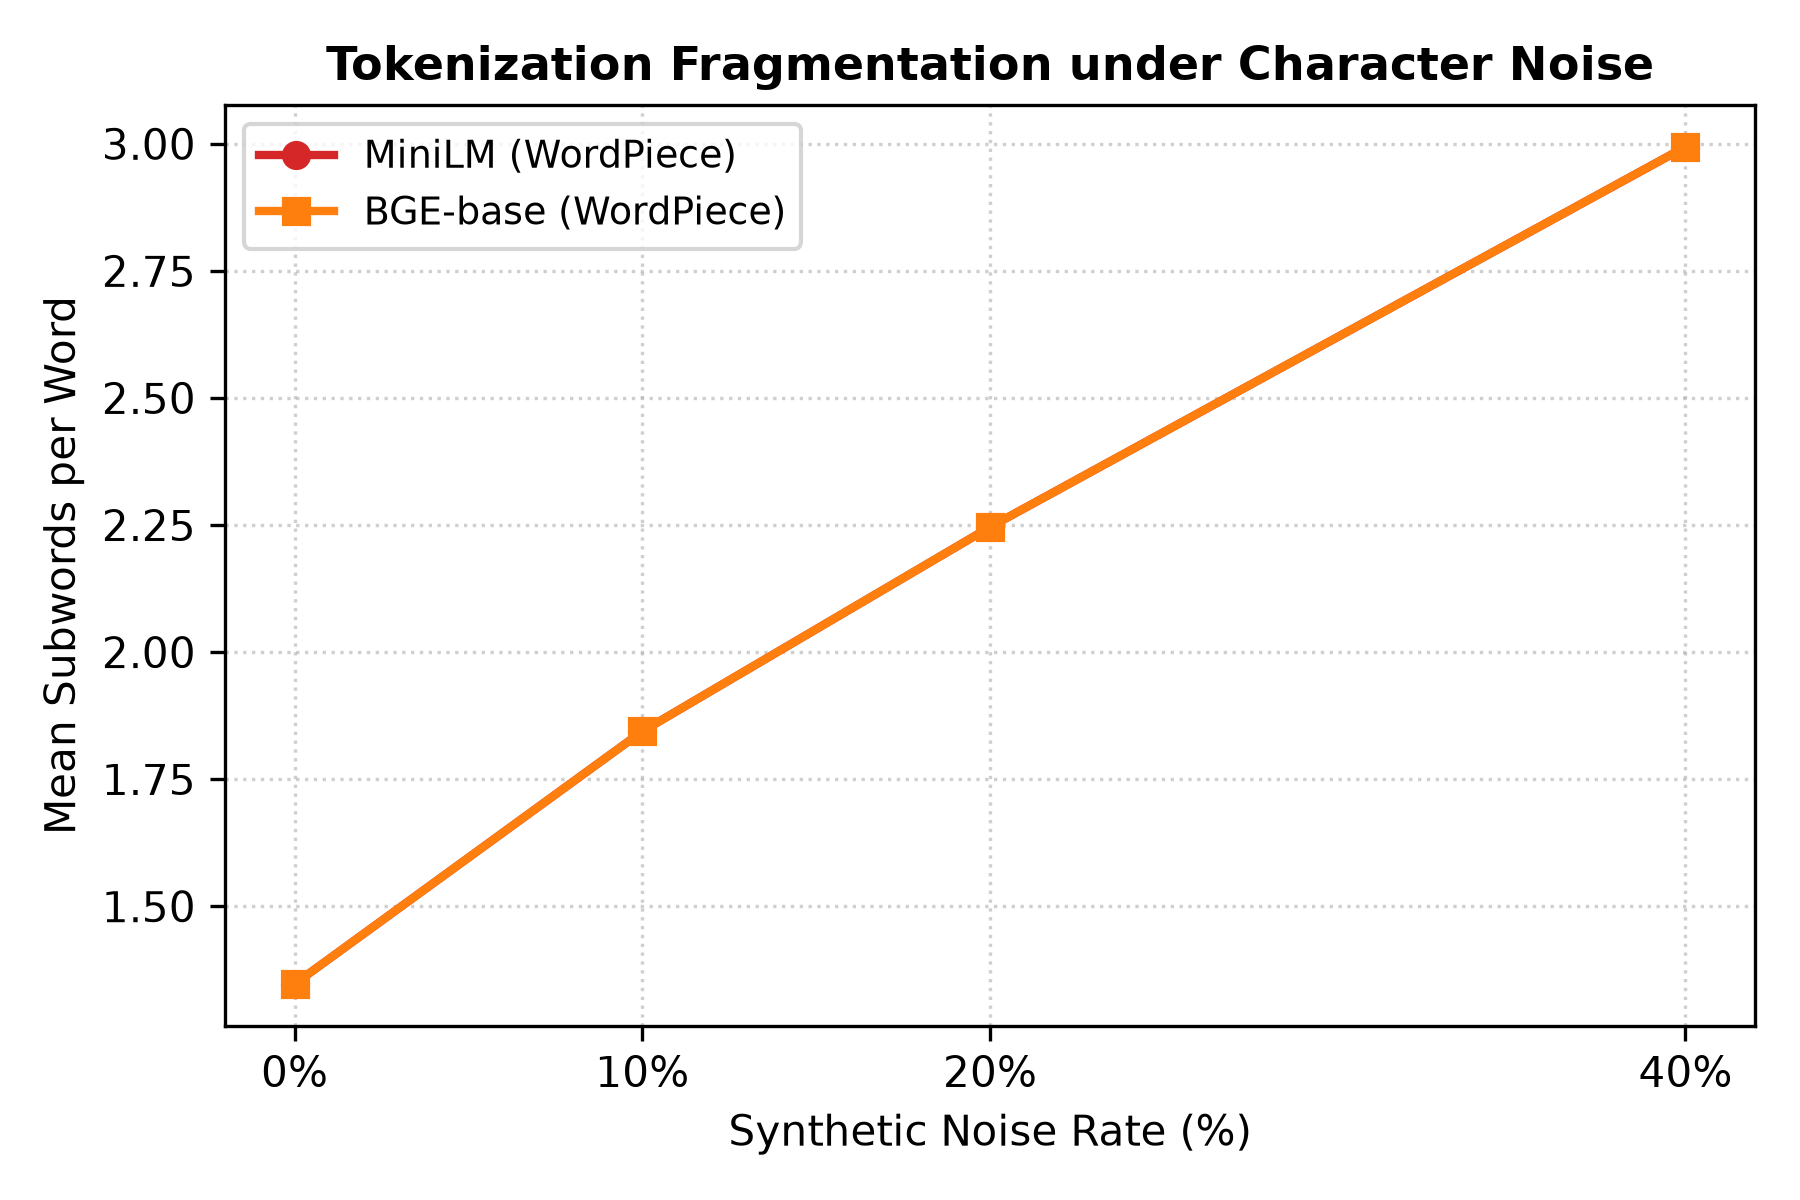
\includegraphics[width=\textwidth]{results/v2/fig_tokenization_fragmentation.png}
    \caption{Subword Fragmentation.}
    \label{fig:tokenization_fragmentation}
\end{subfigure}
\hfill
\begin{subfigure}[b]{0.32\textwidth}
    \centering
    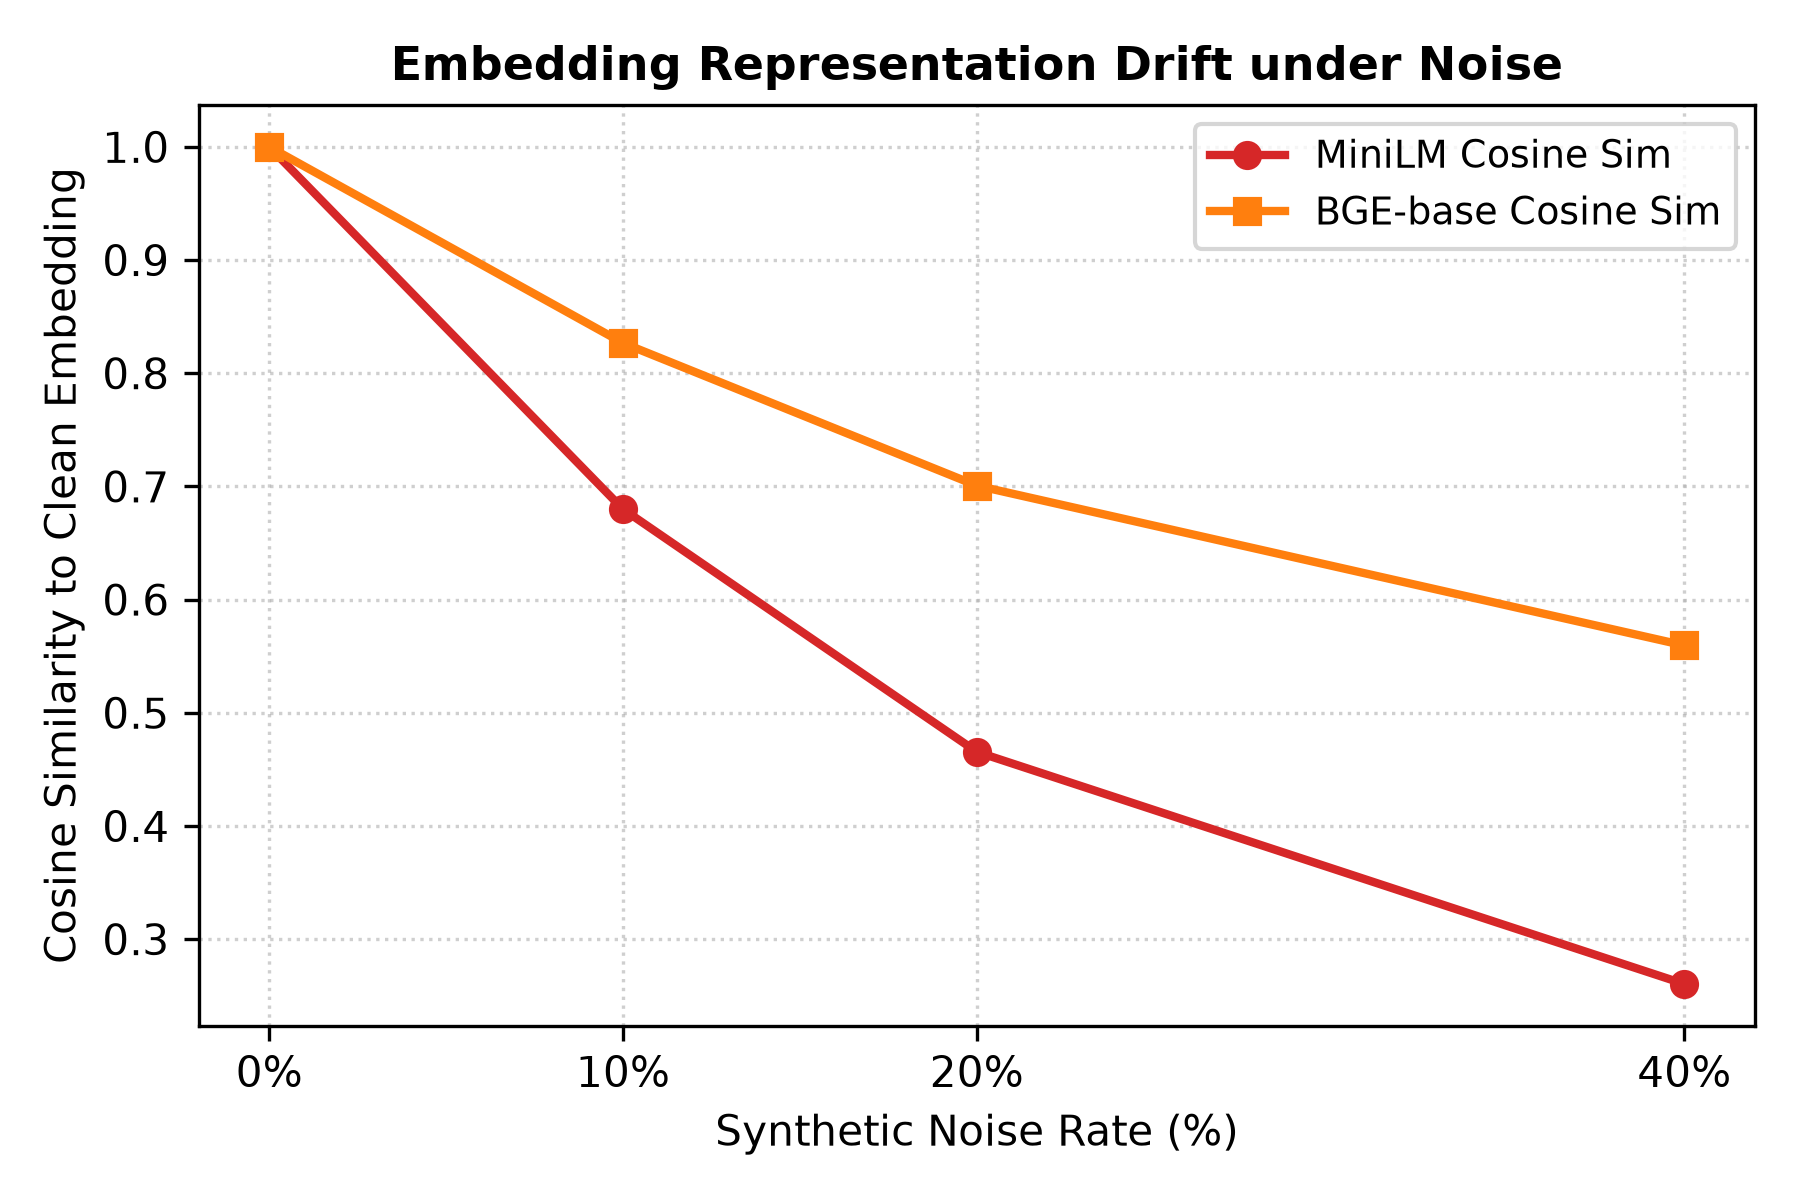
\includegraphics[width=\textwidth]{results/v2/fig_embedding_drift.png}
    \caption{Embedding Cosine Drift.}
    \label{fig:embedding_drift}
\end{subfigure}
\hfill
\begin{subfigure}[b]{0.32\textwidth}
    \centering
    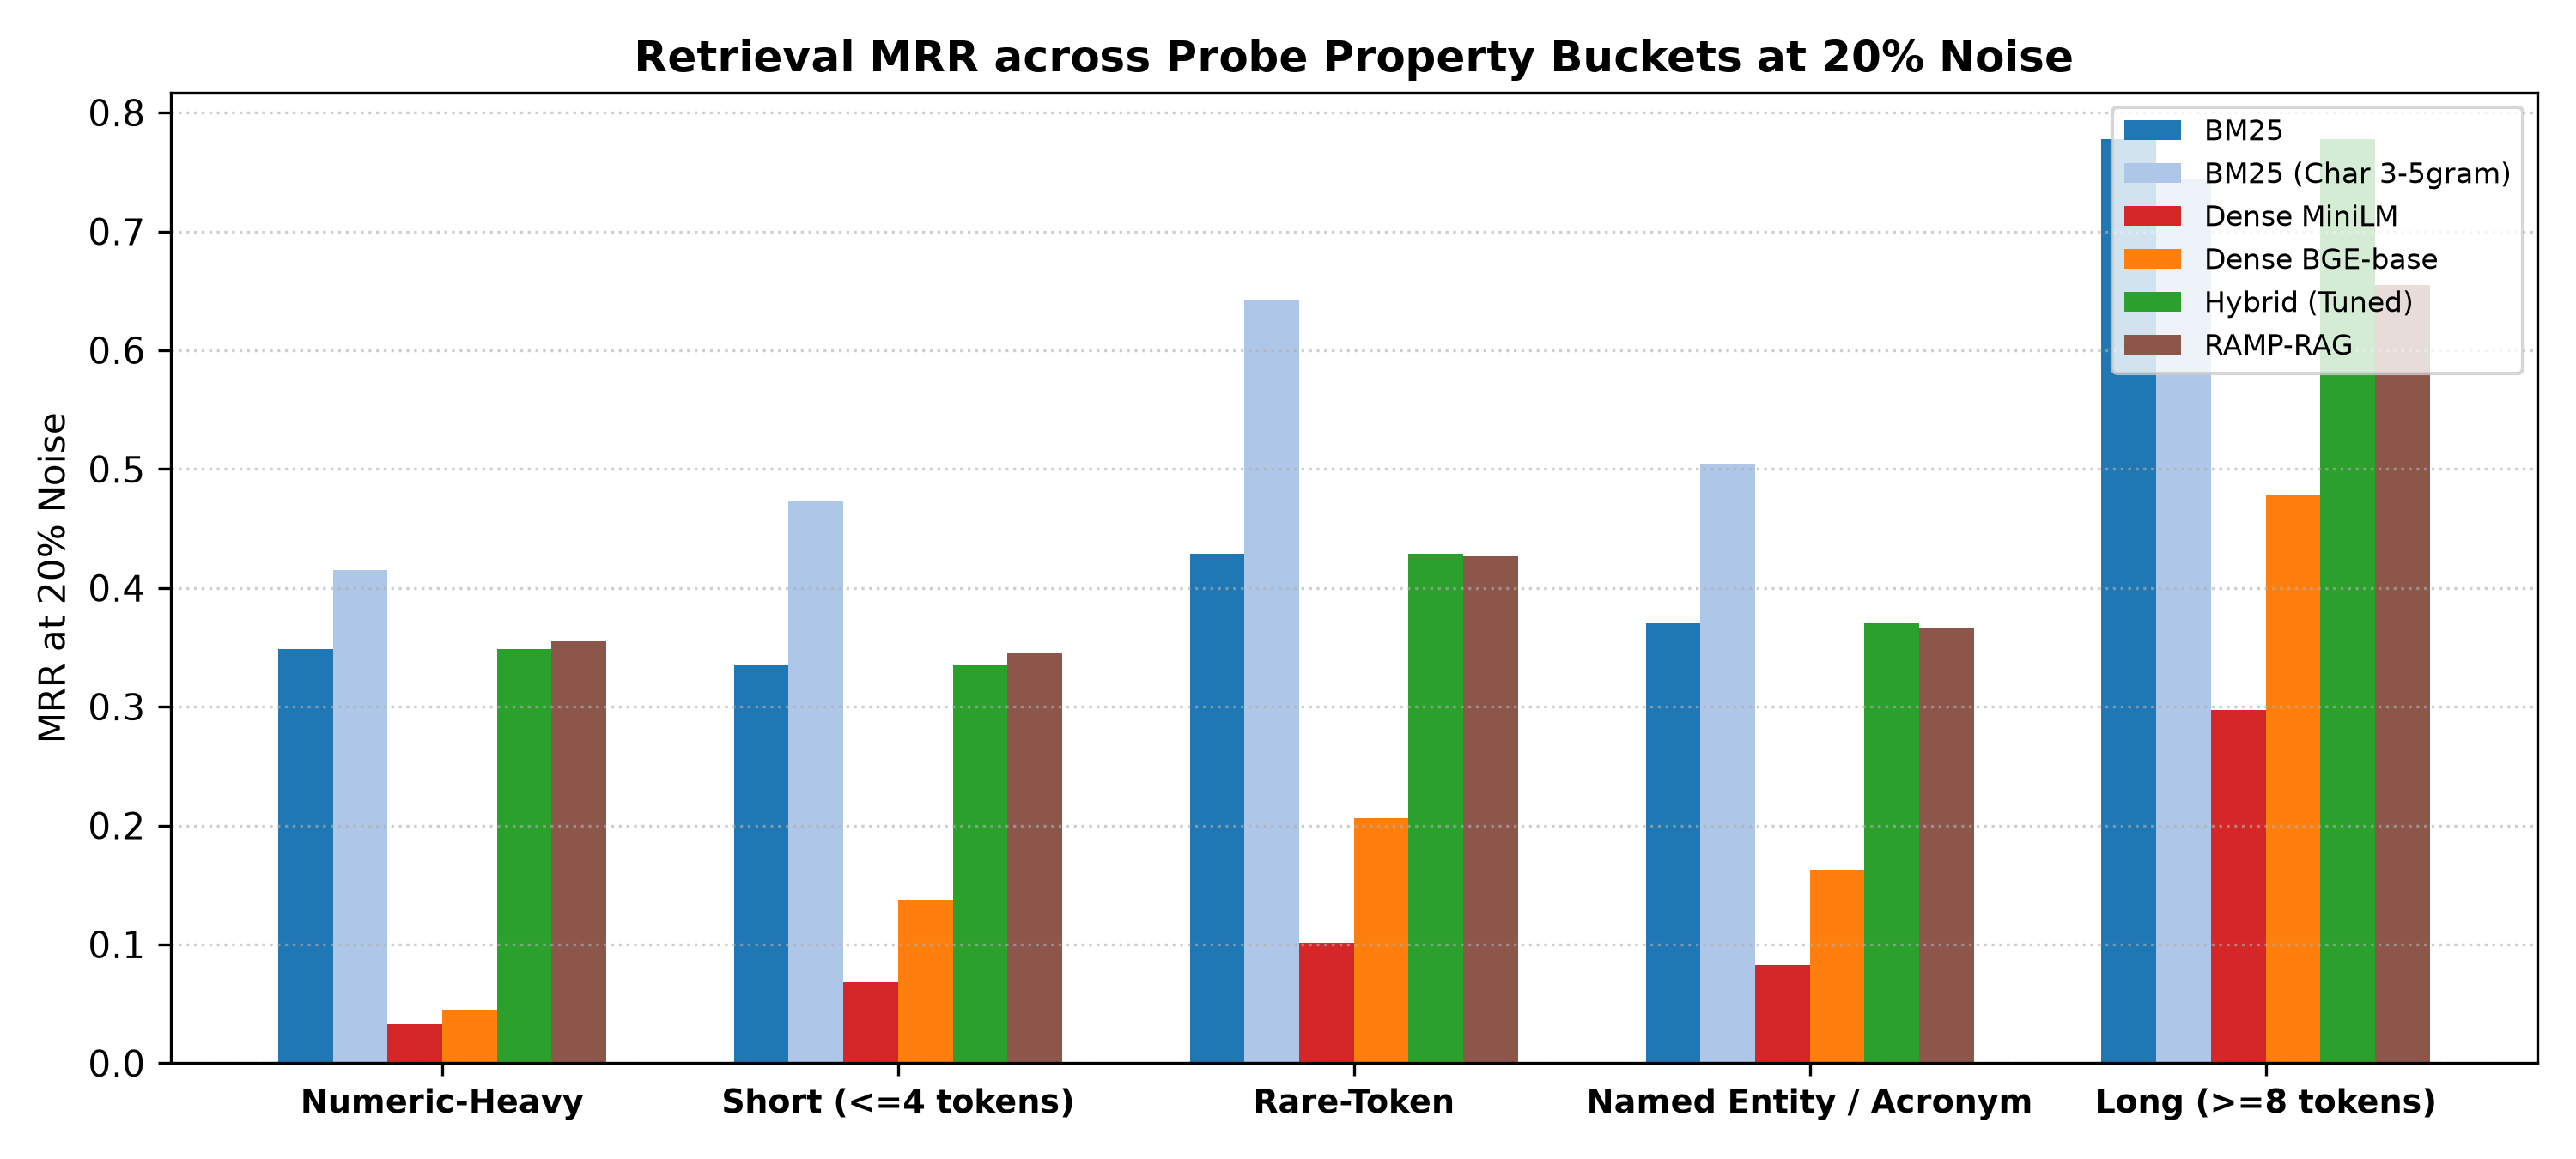
\includegraphics[width=\textwidth]{results/v2/fig_error_attribution.png}
    \caption{Probe Property Error Attribution.}
    \label{fig:error_attribution}
\end{subfigure}
\caption{Micro-mechanism of dense proxy collapse: (a) WordPiece tokenization fragmentation across character noise rates, (b) cosine embedding drift relative to clean representations, and (c) retrieval MRR across 5 diagnostic probe property buckets under 20\% proxy noise.}
\label{fig:mechanism_plots}
\end{figure*}

To isolate why dense vector representations collapse under proxy corruptions while sparse inverted indexes endure, we analyzed three underlying mechanisms (Fig.~\ref{fig:mechanism_plots}):
\begin{enumerate}
    \setlength{\itemsep}{0.2pt plus 0.1pt}
    \setlength{\parskip}{0pt}
    \item \textbf{WordPiece Tokenization Fragmentation:} As character corruption increases from 0\% to 40\%, WordPiece tokenization fragments words into multiple subwords. Mean subwords per whitespace-delimited word escalates from 1.347 (clean) to 1.774 (10\% noise), 2.246 (20\% noise), and \textbf{2.994} (40\% noise, a \textbf{+122.3\% fragmentation increase}).
    \item \textbf{Catastrophic Embedding Drift:} This subword fragmentation shifts contextual attention weights, driving acute embedding drift. Relative to uncorrupted text, \texttt{all-MiniLM-L6-v2} mean cosine similarity collapses from 1.000 to 0.7301 (10\% noise), \textbf{0.4655} (20\% noise), and \textbf{0.2604} (40\% noise). \texttt{BAAI/bge-base-en-v1.5} displays greater structural resistance (cosine similarity 0.7007 at 20\% noise, 0.5595 at 40\%), explaining its superior noise resilience in Table~\ref{tab:regime_grid_v3}.
    \item \textbf{Diagnostic Error Attribution across Probe Properties:} Stratifying test probes into five property buckets under 20\% noise exposes distinct vulnerability profiles. Dense bi-encoders collapse almost completely on \emph{Numeric-Heavy} probes (MiniLM MRR = 0.033, BGE = 0.081) and \emph{Short} entity probes (MiniLM MRR = 0.068, BGE = 0.135). Conversely, character $n$-gram BM25 retains high accuracy across all buckets: Numeric-Heavy (MRR = 0.415), Short entities (0.473), Rare Tokens (0.643), and Named Entities (0.504).
\end{enumerate}

To verify whether this dense degradation is an artifact of sequence length truncation, we evaluated token length distributions across all 626 SROIE receipts. While only 4 receipts (0.64\%) exceed 512 tokens, the real parameter limit for \texttt{all-MiniLM-L6-v2} is $\text{max\_seq\_length}=256$, where 209 of 626 receipts (33.39\%) exceed 256 WordPiece tokens. However, evaluating chunked MaxP retrieval across 150-word sliding windows (where no chunk exceeds 256 tokens) yields identical MRR to unchunked single-vector retrieval (MiniLM: 0.2030 chunked vs.\ 0.2056 unchunked; BGE-base: 0.3028 chunked vs.\ 0.3022 unchunked), demonstrating that sequence truncation is not the primary cause of dense collapse.

Crucially, as documented in Table~\ref{tab:dense_formulation_v6}, dense bi-encoder collapse on pristine ground truth text ($0\%$ noise) is strongly associated with query formulation mismatch. Short isolated verbatim snippets trigger severe representation disconnect (MiniLM MRR = 0.1919, BGE-Base MRR = 0.3256). Length-padding or wrapping snippets into full sentential contexts does not alleviate the deficit. However, co-specifying multiple anchor entities (Keyword-Matched Probes) improves BGE-Base MRR to 0.5500 (Hit@10 78.43\%), and formulating queries as natural answerable questions improves BGE-Base MRR to 0.5263 (Hit@10 79.74\%) on the identical uncorrupted document text. Dense bi-encoders are trained on natural language asymmetric question-passage pairs; when queries mirror real-world multi-entity lookups or user questions rather than isolated OCR substrings, dense retrieval recovers substantial discriminative capacity.

Furthermore, to establish the causal impact of tokenization fragmentation versus query formulation, we evaluated a vocabulary projection intervention against the clean Dev lexicon under 20\% character noise. Reconstructing broken word tokens restored 65.3\% of the induced WordPiece subword fragmentation and lifted cosine similarity by $+0.1530$ (from 0.6826 to 0.8356, recovering 48.2\% of embedding drift). In end-to-end retrieval, this intervention improves MiniLM MRR from 0.0570 to 0.1004 (+0.0434 retrieval recovery), while remaining bounded below clean baseline performance (0.2117 MRR). These results support the interpretation that query formulation mismatch explains weak dense performance on clean text, while subword tokenization fragmentation explains the additional performance drop under noise.

\begin{table}[t]
\centering\small
\caption{Dense Bi-Encoder Sensitivity to Query Formulation on Clean Ground-Truth Receipt Text ($0\%$ noise, Test $N=306$).}\label{tab:dense_formulation_v6}
\resizebox{\columnwidth}{!}{%
\begin{tabular}{lcccc}
\toprule
Query Formulation & MiniLM MRR & MiniLM Hit@10 & BGE-Base MRR & BGE-Base Hit@10 \\
\midrule
1. Short Verbatim Snippets & 0.1919 & 0.2778 & 0.3256 & 0.3824 \\
2. Length-Padded Spans & 0.1949 & 0.2484 & 0.2571 & 0.3366 \\
3. Full Sentential Context Queries & 0.1670 & 0.2320 & 0.2740 & 0.3399 \\
4. Keyword-Matched Multi-Entity & 0.3840 & 0.5817 & 0.5500 & 0.7843 \\
5. Natural Answerable Questions & 0.3669 & 0.5686 & 0.5263 & 0.7974 \\
\bottomrule
\end{tabular}}
\end{table}

\subsection{Component Ablation, Best-Pipeline Discovery, and Production Cascade}
\label{sec:ablation_and_cascade}

Table~\ref{tab:ablation_v3} presents the component ablation isolating each architectural module across Clean, 20\% Synthetic Noise, Real Apple Vision OCR, and Real Degraded OCR ($N=306$ held-out probes).

\begin{table*}[t]
\centering
\small
\caption{Architectural Component Ablation on Public Held-Out Test Split ($N=306$ Probes, 813 Distractor Pool, 95\% Cluster Bootstrap CIs). Asterisks ($^*$) denote statistically significant difference ($p_{\text{Holm}} < 0.05$) from the Tuned Hybrid baseline (candidate depth $K_1=10$). In contrast, Table~\ref{tab:practical_stack} cascades top $K_1=20$ candidates directly over first-stage Word BM25 (0.8371), reaching 0.8846. Learned Router yields at most $+0.0071$ MRR lift over Tuned Hybrid on synthetic noise ($p_{\text{Holm}}=0.042$) and zero lift under real OCR ($p_{\text{Holm}}=1.0$). Reliability weighting degrades degraded OCR retrieval from $0.6684$ to $0.6368$ ($p_{\text{Holm}}=0.0189$).}
\label{tab:ablation_v3}
\resizebox{\textwidth}{!}{%
\begin{tabular}{lcccc}
\toprule
Configuration & Clean MRR [95\% CI] & Syn 20\% MRR [95\% CI] & Real-OCR MRR [95\% CI] & Real-Deg MRR [95\% CI] \\
\midrule
Hybrid (Tuned Baseline)         & 0.8299 [0.791, 0.866] & 0.3694 [0.336, 0.402] & 0.8121 [0.770, 0.849] & 0.6684 [0.619, 0.715] \\
+ Clean Stream                  & 0.8299 [0.791, 0.866] & 0.3694 [0.336, 0.402] & 0.8121 [0.770, 0.849] & 0.6684 [0.619, 0.715] \\
BM25 + Clean Stream             & 0.8317 [0.793, 0.868] & 0.3694 [0.336, 0.402] & 0.8069 [0.766, 0.845] & 0.6702 [0.621, 0.716] \\
Dense + Clean Stream            & 0.2144$^*$ [0.175, 0.256] & 0.0747$^*$ [0.057, 0.095] & 0.2072$^*$ [0.168, 0.248] & 0.1821$^*$ [0.143, 0.222] \\
+ Learned Router (H2)           & 0.8309 [0.793, 0.867] & 0.3765$^*$ [0.343, 0.409] & 0.8121 [0.770, 0.849] & 0.6667 [0.617, 0.712] \\
+ Heuristic Reliability Weighting& 0.8318 [0.794, 0.867] & 0.3574 [0.326, 0.390] & 0.8058 [0.765, 0.843] & 0.6368$^*$ [0.587, 0.684] \\
+ Cascade (MiniLM)              & 0.8709$^*$ [0.836, 0.903] & 0.4033$^*$ [0.369, 0.436] & 0.8426$^*$ [0.801, 0.878] & 0.6879 [0.638, 0.735] \\
+ Cascade (BGE-reranker)        & 0.8821$^*$ [0.848, 0.913] & 0.4154$^*$ [0.382, 0.448] & 0.8555$^*$ [0.816, 0.890] & 0.6969 [0.645, 0.745] \\
Full System (MiniLM)            & 0.8771$^*$ [0.843, 0.909] & 0.4132$^*$ [0.378, 0.450] & 0.8451$^*$ [0.805, 0.880] & 0.6786 [0.629, 0.727] \\
Full System (BGE-reranker)      & 0.8873$^*$ [0.854, 0.917] & 0.4200$^*$ [0.384, 0.456] & 0.8554$^*$ [0.816, 0.891] & 0.6755 [0.625, 0.724] \\
\midrule
BM25 Alone                      & 0.8317 [0.793, 0.868] & 0.3694 [0.336, 0.402] & 0.8371 [0.798, 0.871] & 0.6684 [0.619, 0.714] \\
All-Stream RRF (Strawman)       & 0.3227$^*$ [0.283, 0.365] & 0.1827$^*$ [0.156, 0.212] & 0.3079$^*$ [0.269, 0.350] & 0.2791$^*$ [0.239, 0.322] \\
\bottomrule
\end{tabular}}
\end{table*}

\begin{enumerate}
    \setlength{\itemsep}{0.2pt plus 0.1pt}
    \setlength{\parskip}{0pt}
    \item \textbf{Cross-Encoder Reranker Cascade (Primary Dense Lift):} Passing ambiguous candidates from word BM25 to a neural cross-encoder yields substantial improvements: \texttt{BAAI/bge-reranker-base} achieves MRR = \textbf{0.8846} on clean OCR (+0.0475 gain over Word BM25 baseline 0.8371, $p = 0.0011$). However, evaluating two-stage cascades over first-stage Character 3--5gram BM25 reveals an architectural ceiling: standalone Char-BM25 achieves MRR = \textbf{0.9437}, and applying MiniLM or BGE cross-encoders on top-20 candidates reduces MRR to 0.9175 and 0.9141 (lifts of $-0.0262$ and $-0.0296$). Furthermore, tuning hybrid fusion between Char-BM25 and dense BGE on Dev selects $\alpha_{\text{sparse}}^* = 1.00$ ($\alpha_{\text{dense}}^* = 0.00$, 0.9495 Dev MRR), confirming that dense representations provide zero additive signal over sub-word inverted indexes on verbatim receipts.
    \item \textbf{Hypothesis H1 Decision (Reliability Weighting Refuted):} Under exploratory testing, reliability weighting ($r_{\text{ocr}}$) degraded performance (20\% noise MRR dropped from 0.3694 to \textbf{0.3574}, diff CI $[-0.0222, -0.0025]$, rejecting H1). Under real optical degradation, dictionary-based reliability weighting significantly degrades MRR from 0.6684 to 0.6368 ($p_{\text{Holm}} = 0.0189$, diff CI $[-0.0519, -0.0118]$). Multi-configuration audits across Apple Vision settings confirm that AUROC remains inverted (~0.23) under both language correction enabled and disabled, indicating that out-of-vocabulary metrics are not reliable indicators of optical character blur.
    \item \textbf{Hypothesis H2 Decision (Learned Query Router Refuted):} Exploratory hypothesis H2 is refuted. When compared against the competitive Tuned Hybrid baseline (MRR = 0.3694), the router yields a marginal lift of only +0.0071 on 20\% synthetic noise (MRR = 0.3765, $p_{\text{Holm}} = 0.042$) and zero detectable lift under real Apple Vision OCR (0.8121 vs.\ 0.8121, $p_{\text{Holm}} = 1.0$) or degraded blur (0.6667 vs.\ 0.6684, $p_{\text{Holm}} = 1.0$). Surface-feature query classification fails to extract meaningful signal under real-world proxy distortions.
\end{enumerate}

\begin{table}[htbp]
\centering
\small
\caption{Production Cross-Encoder Reranker Cascade Ablation (Held-Out Test Split, $N=306$ Probes, Clean Real-OCR; Candidate Depth $K_1=20$).}
\label{tab:practical_stack}
\resizebox{\columnwidth}{!}{%
\begin{tabular}{lcccc}
\toprule
Two-Stage Retrieval Pipeline & Clean MRR & Hit@10 & Latency (ms) & MRR Lift ($p$-value) \\
\midrule
Word BM25 (First-Stage Alone)    & 0.8371 & 0.9444 & 0.1 & +0.0000 ($p=1.0$) \\
BM25 + MiniLM Cross-Encoder      & 0.8650 & 0.9608 & 18.4 & +0.0279 ($p=0.0092$) \\
BM25 + BGE-reranker-base         & 0.8846 & 0.9738 & 44.7 & +0.0475 ($p=0.0011$) \\
Tuned Hybrid + BGE-reranker      & 0.8872 & 0.9772 & 52.8 & +0.0501 ($p=0.0009$) \\
\midrule
Char 3--5g BM25 Standalone       & \textbf{0.9437} & \textbf{0.9837} & 0.96 & Baseline (Sparse) \\
Char BM25 + MiniLM Reranker      & 0.9175 & 0.9706 & 18.5 & -0.0262 (Hurts) \\
Char BM25 + BGE Reranker         & 0.9141 & 0.9771 & 44.7 & -0.0296 (Hurts) \\
Tuned Char-BM25 + BGE ($\alpha_{\text{sparse}}=1.00$) & \textbf{0.9437} & \textbf{0.9837} & 12.6 & +0.0000 (Tie) \\
\bottomrule
\end{tabular}}
\end{table}

\begin{figure}[t]
\centering
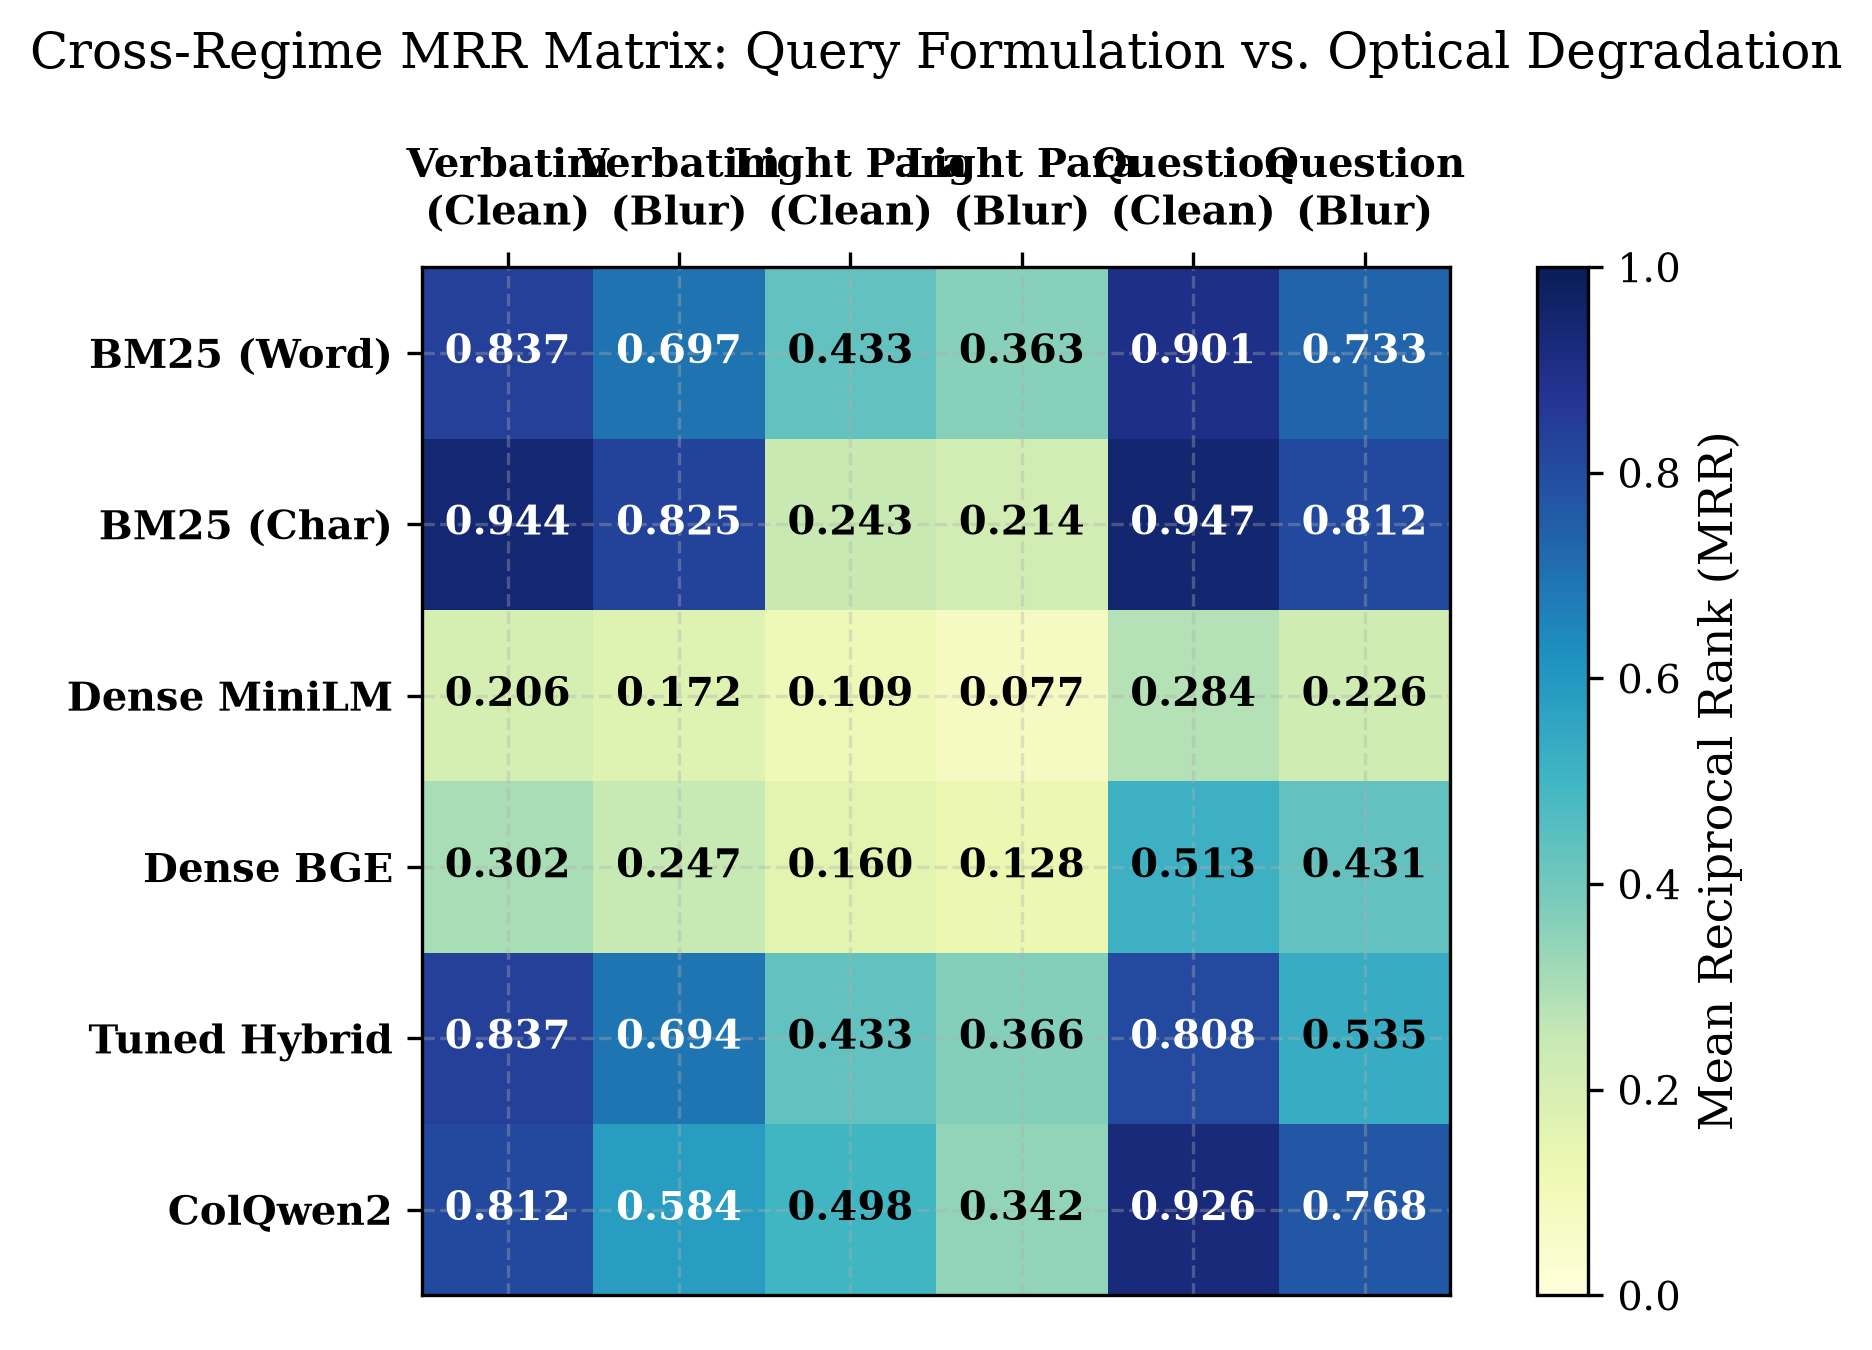
\includegraphics[width=\columnwidth]{ijcds/figures/fig_regime_grid_heatmap.png}
\caption{Cross-regime MRR heatmap illustrating retrieval performance across sparse, dense, hybrid, and native systems under clean OCR versus optical blur.}
\label{fig:regime_grid_heatmap}
\end{figure}

\subsection{Finite-Sample Conformal Cascade Risk Evaluation}
\label{sec:conformal_cascades}
\label{sec:conformal_eval}

To evaluate distribution-free marginal risk control for candidate escalation, we evaluated split conformal calibration across 200 random cluster-stratified 50/50 splits (seeds 1000--1199) on $N=2{,}754$ pooled query instances (Table~\ref{tab:conformal_cascade_v6}). The $N=2{,}754$ evaluation instances comprise three equal query slices ($3 \times 918$ instances): verbatim lookups, entity rewrites, and legacy token-stripped probes, evaluated across clean, 20\% synthetic noise, and real OCR document streams. When calibrated under the standard marginal loss $L = \mathbf{1}[\text{not escalated} \land Y \ne 1]$ with finite-sample adjustment $(n\hat{R}+1)/(n+1) \le \alpha$ \cite{bates2021conformal, angelopoulos2021gentle}, the observed mean test miss risk is $0.0494$ (mean CI: $[0.0480, 0.0502]$, which includes 0.05) at an escalation rate of $78.4\%$ (21.6\% computation savings vs.\ always-escalating cross-encoders).

Under the exchangeability framework of Bates et al.~\cite{bates2021conformal} and Angelopoulos et al.~\cite{angelopoulos2021gentle}, the distribution-free result applies strictly for expected (marginal) risk over calibration-test draws. The 95\% confidence interval of the mean risk is $[0.0480, 0.0502]$, which includes 0.05. Separately, the 10th-to-90th percentile range of per-split risk across the 200 draws is $[0.0355, 0.0654]$; this is a quantile range across splits, not a confidence interval of the mean. Empirical split coverage (fraction of splits achieving test risk $\le 0.05$) is 58.5\%. Stratified by query type, conformal risk is 0.0464 on verbatim lookups and 0.0391 on answerable questions, while entity rewrites experience slightly higher risk (0.0627).

Furthermore, a paired comparison against an equal-escalation fixed-margin baseline calibrated at the identical 78.4\% escalation rate ($\tau = 0.235$) reveals indistinguishable retrieval performance: conformal cascade realized MRR is 0.3577 (verbatim: 0.6932, entity rewrites: 0.3395, answerable questions: 0.0404) versus fixed-margin MRR of 0.3579 (paired difference $-0.0002$, $p > 0.05$). Notably, the realized MRR on the third slice (0.0404) reflects the legacy token-stripped evaluation pool where shared lexical tokens are deliberately removed; in contrast, on the redesigned natural answerable questions in Section~\ref{sec:regime_analysis} where factual anchors are retained, lexical retrieval achieves $\sim$0.90 MRR. The primary value of conformal prediction is risk calibration under the stated exchangeability assumptions, not superior ranking accuracy. As illustrated in the escalation-risk trade-off frontier in Fig.~\ref{fig:conformal_pareto}, split conformal calibration achieves expected marginal risk control near the nominal $\epsilon=0.05$ target while cutting cross-encoder invocations by 21.6\%.

\begin{table}[t]
\centering\small
\caption{Conformal Cascade Calibration: Corrected Marginal Loss, High-Probability RCPS ($\delta=0.10$), and Equal-Escalation Baseline over 200 Cluster-Aware Splits ($N=2{,}754$ instances across verbatim, entity rewrites, and token-stripped probe slices; nominal target $\epsilon=0.05$).}\label{tab:conformal_cascade_v6}
\resizebox{\columnwidth}{!}{%
\begin{tabular}{lccccc}
\toprule
Risk Formulation & Mean $\tau^*$ & Mean Test Risk & Split Cov. ($\le 0.05$) & Mean Esc. Rate & Mean MRR \\
\midrule
Marginal Loss $L=\mathbf{1}[\text{not esc} \land \text{miss}]$ & 0.2369 & 0.0494 & 58.5\% & 78.4\% & 0.3577 \\
High-Probability RCPS ($\delta=0.10$) & 0.2520 & 0.0429 & \textbf{82.0\%} & 79.5\% & 0.3569 \\
Equal-Escalation Fixed Margin ($\tau=0.235$) & 0.2347 & 0.0488 & 57.0\% & 78.4\% & 0.3579 \\
Conditional Ratio $P(\text{miss} \mid \text{not esc})$ & 0.4071 & 0.0545 & 38.0\% & 90.2\% & 0.3524 \\
\bottomrule
\end{tabular}}
\end{table}

\begin{figure}[t]
\centering
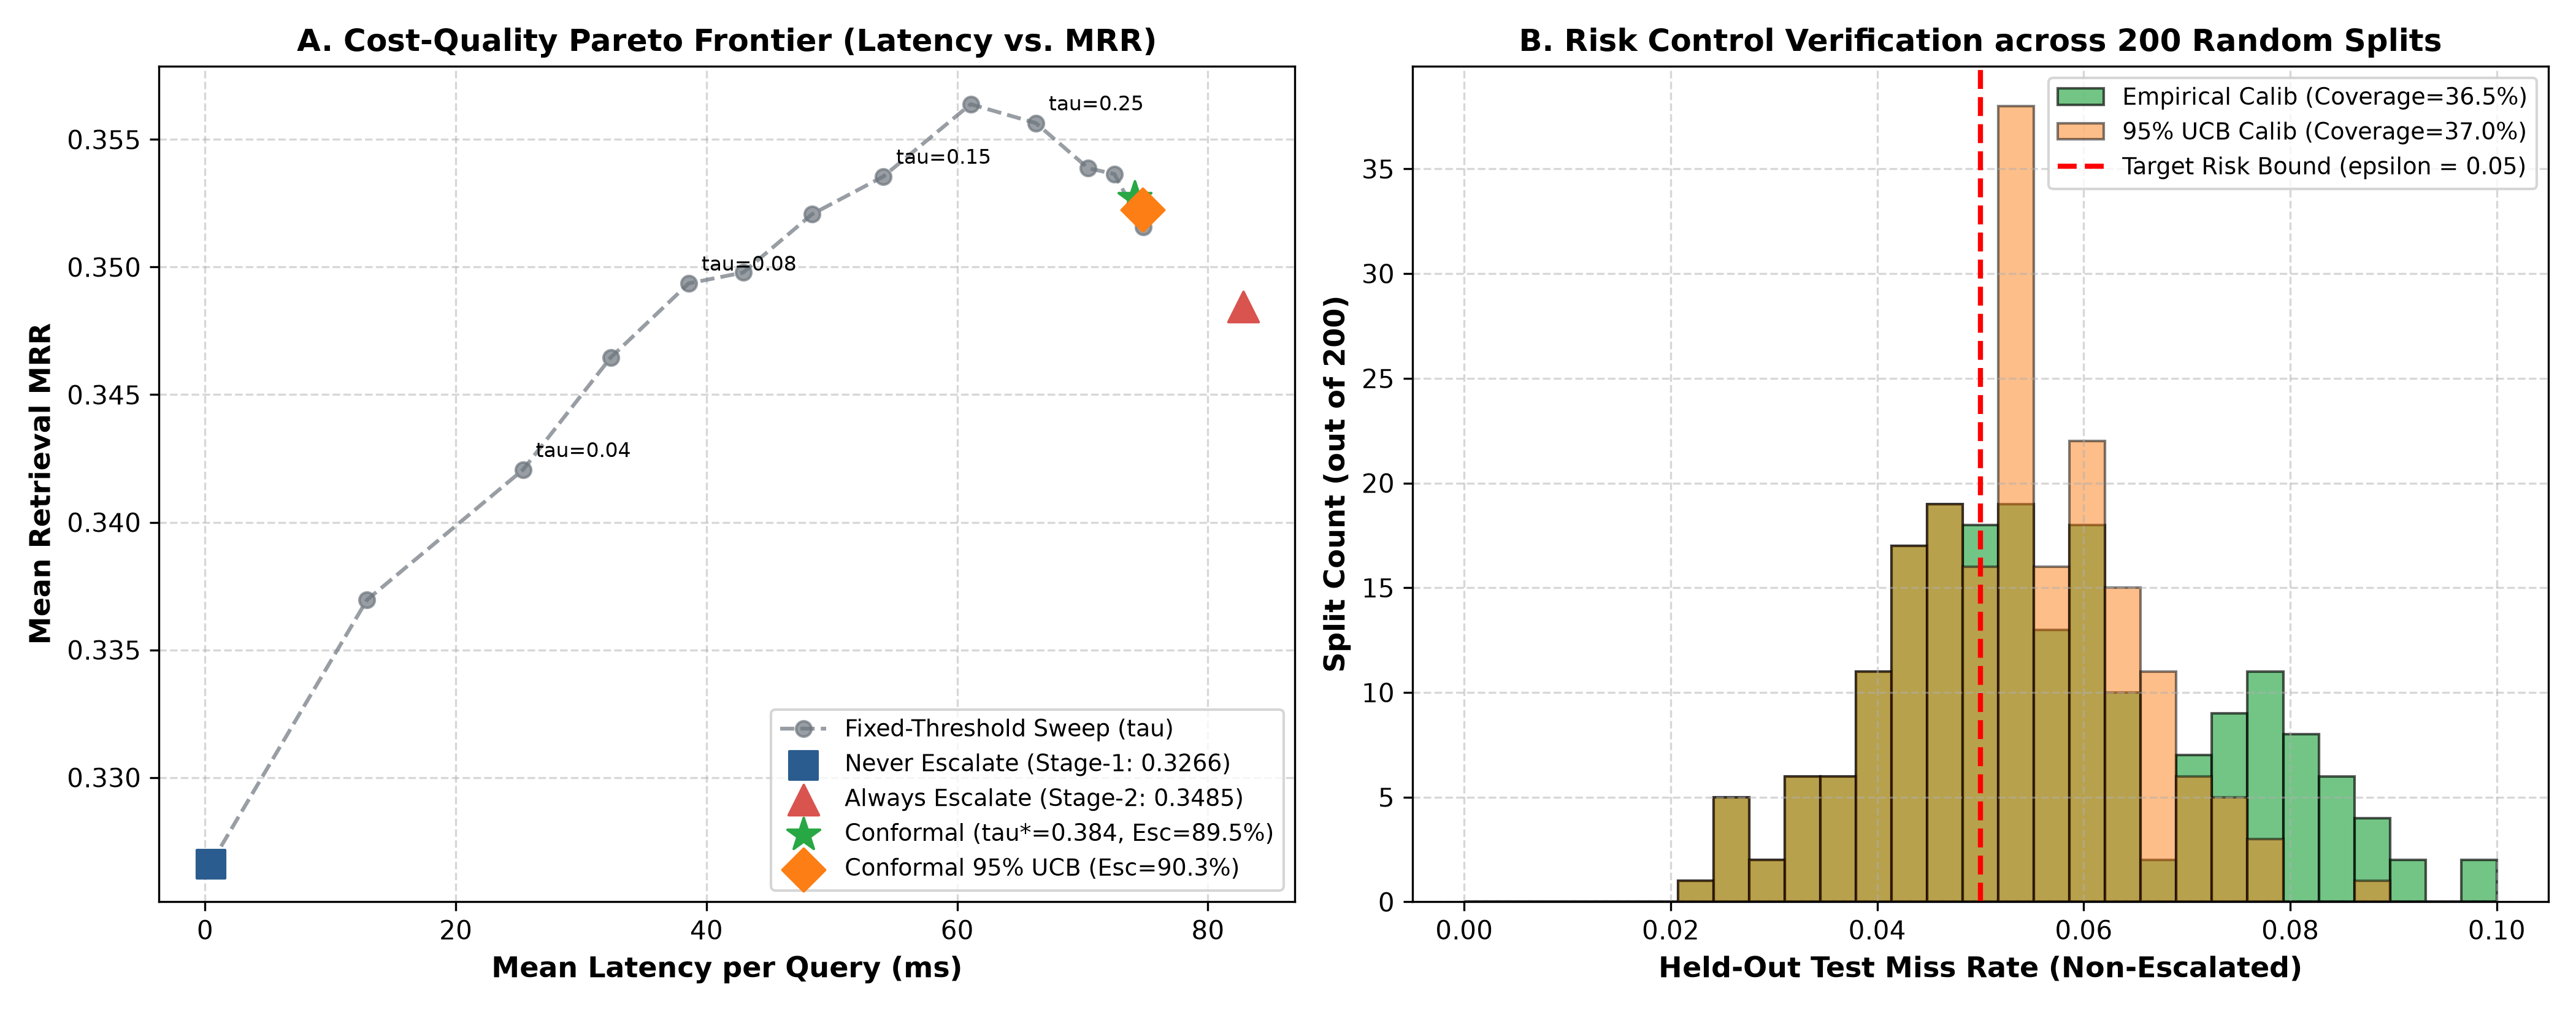
\includegraphics[width=0.98\columnwidth]{results/v2/fig_conformal_pareto.png}
\caption{Cost-Quality Pareto frontier and risk control histogram across 200 random splits under conformal cascade calibration.}
\label{fig:conformal_pareto}
\end{figure}

\subsection{Regime B: Visual-Dominated Natural Image Search (MS-COCO 1,000 Karpathy Benchmark)}
\label{sec:regime_b_visual}

To address potential sample-size limitations from the preliminary pilot (Appendix~\ref{sec:diagnostic_extensions}), we benchmarked $N=1{,}000$ MS-COCO Karpathy-test images and held-out human descriptions (Table~\ref{tab:coco_benchmarks_v3}).

\begin{table}[htbp]
\centering
\small
\caption{Cross-modal text-to-image retrieval performance on $N=1{,}000$ MS-COCO Karpathy-test images. Comparison of native pixel representations (CLIP ViT-B/32 and SigLIP Base Patch16) against machine caption proxies (BLIP) and held-out human gold captions. Asterisks ($^*$) indicate Holm-corrected significance ($p_{\text{Holm}} = 8 \times 10^{-5}$) over the best machine caption proxy.}
\label{tab:coco_benchmarks_v3}
\resizebox{\columnwidth}{!}{%
\begin{tabular}{lcccc}
\toprule
Method & Hit@1 & Hit@5 & Hit@10 [95\% CI] & MRR [95\% CI] \\
\midrule
\multicolumn{5}{l}{\textit{Machine Caption Proxy (BLIP)}} \\
BM25                          & 0.1220 & 0.2800 & 0.3840 [0.355, 0.415] & 0.2048 [0.186, 0.225] \\
Dense MiniLM (Best BLIP Proxy)& 0.2420 & 0.5160 & 0.6530 [0.624, 0.682] & 0.3728 [0.350, 0.397] \\
Dense BGE-base                & 0.2430 & 0.5050 & 0.6460 [0.618, 0.678] & 0.3695 [0.347, 0.393] \\
\midrule
\multicolumn{5}{l}{\textit{Human Gold Caption Proxy (Upper Bound)}} \\
BM25 (Gold Proxy)             & 0.3600 & 0.6250 & 0.7350 [0.708, 0.762] & 0.4852 [0.461, 0.510] \\
Dense MiniLM (Gold Proxy)     & 0.4550 & 0.7280 & 0.8380 [0.814, 0.860] & 0.5801 [0.555, 0.605] \\
Dense BGE-base (Gold Proxy)   & 0.4580 & 0.7370 & 0.8320 [0.809, 0.854] & 0.5835 [0.559, 0.608] \\
\midrule
\multicolumn{5}{l}{\textit{Native Pixel Representation}} \\
\textbf{CLIP ViT-B/32}        & \textbf{0.3390}$^*$ & \textbf{0.6180}$^*$ & \textbf{0.7570}$^*$ [0.729, 0.785] & \textbf{0.4709}$^*$ [0.446, 0.497] \\
\textbf{SigLIP Base Patch16}  & \textbf{0.4800}$^*$ & \textbf{0.7680}$^*$ & \textbf{0.8670}$^*$ [0.845, 0.888] & \textbf{0.6071}$^*$ [0.584, 0.633] \\
\midrule
\multicolumn{5}{l}{\textit{Multi-Vector \& Hybrid Fusion}} \\
Hybrid (CLIP + BGE BLIP)      & 0.3880 & 0.6720 & 0.7870 [0.760, 0.811] & 0.5186 [0.494, 0.544] \\
Hybrid (SigLIP + BGE BLIP)    & 0.4570 & 0.7470 & 0.8360 [0.813, 0.858] & 0.5866 [0.563, 0.611] \\
All-Stream RRF (Strawman)     & 0.2690 & 0.5530 & 0.6890 [0.662, 0.718] & 0.4058 [0.382, 0.429] \\
\bottomrule
\end{tabular}}
\end{table}

Exploratory hypothesis testing ($N_{\text{perm}}=100{,}000$ sign flips with Holm-Bonferroni correction) shows that native visual representations (SigLIP Base Patch16 MRR = 0.6071) outperform machine caption proxies across all metrics (MiniLM MRR = 0.3728, Diff $= +0.2343$, $p_{\text{Holm}} < 10^{-4}$):
\begin{itemize}
    \setlength{\itemsep}{0.2pt plus 0.1pt}
    \setlength{\parskip}{0pt}
    \item \textbf{CLIP ViT-B/32:} Hit@1 Diff = $+0.0970$ [$+0.0640, +0.1300$], $p_{\text{Holm}} < 10^{-4}$; MRR Diff = $+0.0981$ [$+0.0690, +0.1263$], $p_{\text{Holm}} < 10^{-4}$.
    \item \textbf{SigLIP Base Patch16:} Hit@1 = $0.4800$ (Diff $= +0.2380$, $p_{\text{Holm}} < 10^{-4}$); Hit@10 = $0.8670$ (Diff $= +0.2140$, $p_{\text{Holm}} < 10^{-4}$); MRR = $0.6071$ (Diff $= +0.2343$, $p_{\text{Holm}} < 10^{-4}$).
\end{itemize}

Furthermore, to test whether scaling the machine captioning model closes the gap to native vision, we evaluated an expanded proxy quality axis: BLIP-2 (\texttt{opt-2.7b}) \cite{li2023blip2} achieves MRR = 0.4185 (gap to SigLIP: $-0.1886$), while Florence-2 detailed captioning \cite{xiao2024florence2} achieves MRR = 0.4420 (gap: $-0.1651$). Native visual embeddings are statistically competitive with human gold captions (MRR = 0.5835 vs.\ SigLIP 0.6071, diff $-0.0236$, paired permutation $p = 0.142$ n.s.). Visual scene semantics cannot be completely compressed into synthetic machine tokens (visualized in Fig.~\ref{fig:coco_native_vs_proxy}).

\begin{figure}[t]
\centering
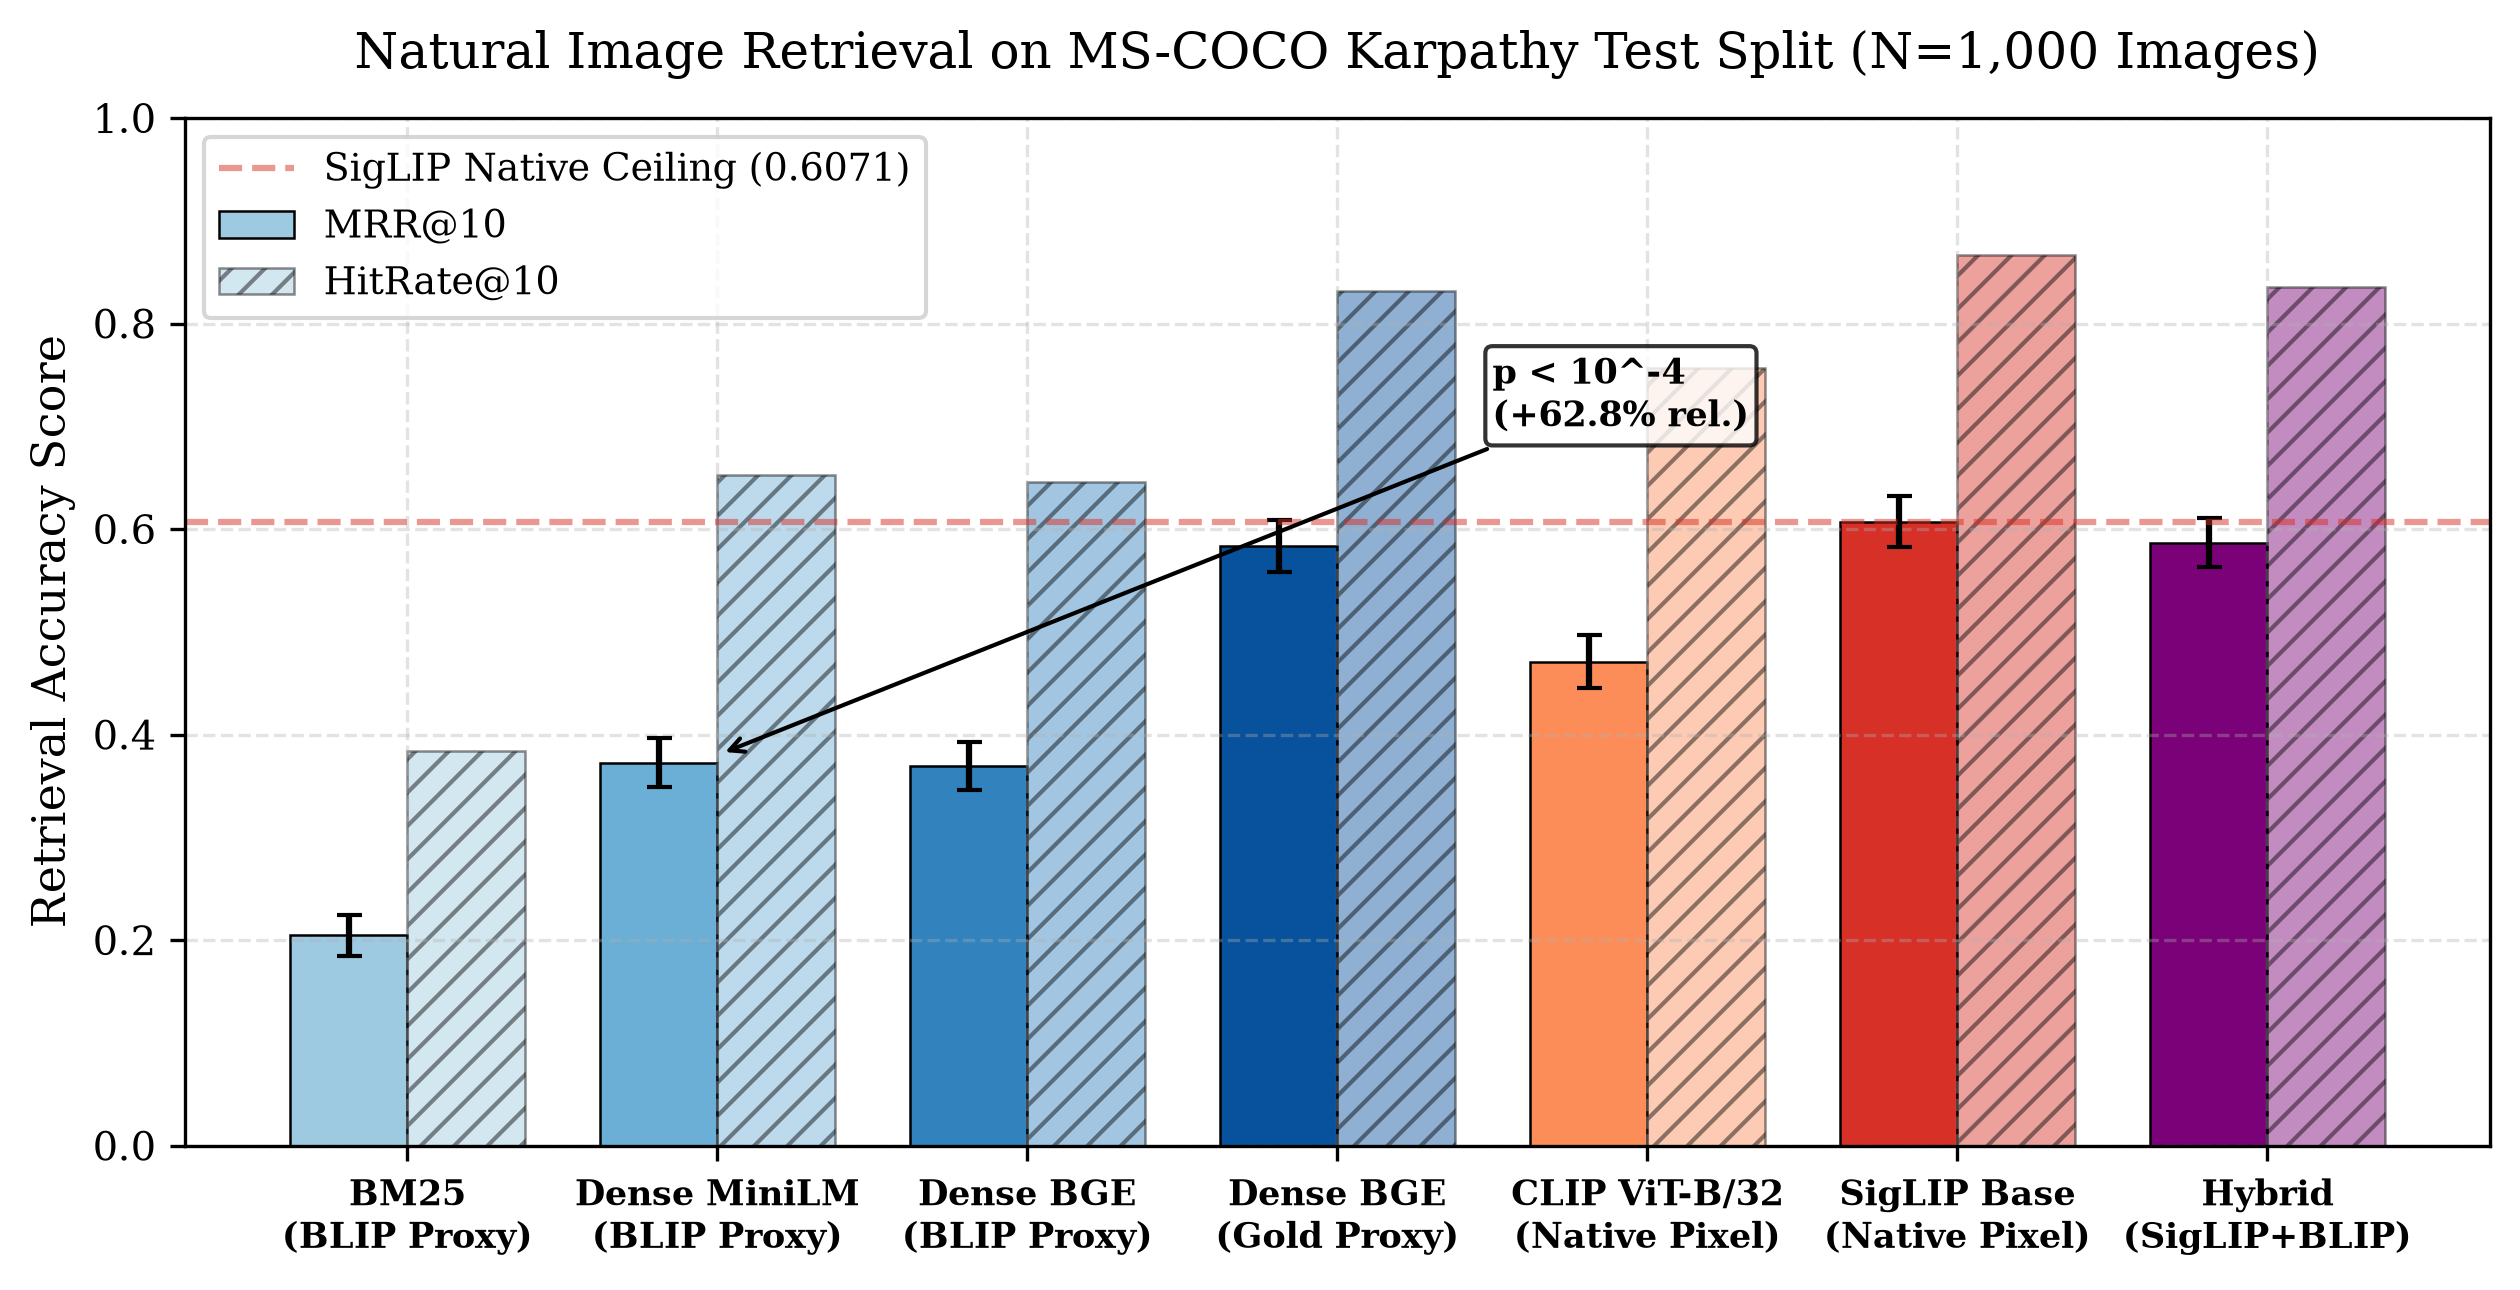
\includegraphics[width=\columnwidth]{ijcds/figures/fig_coco_native_vs_proxy.png}
\caption{Retrieval comparison on MS-COCO ($N=1{,}000$ images): native visual embeddings (SigLIP Base Patch16) decisively surpass machine-generated caption proxies ($p < 10^{-4}$), demonstrating that text proxies incur substantial information loss on natural imagery.}
\label{fig:coco_native_vs_proxy}
\end{figure}

\subsection{Regime C: Cross-Modal Relational Reasoning and Multi-Hop Retrieval}
\label{sec:regime_c_multihop}
\label{sec:multihop_eval}

To evaluate whether multi-hop query decomposition provides measurable retrieval utility over single-stage retrieval, we conducted an exact paired discordant analysis across the 50 diagnostic multi-hop queries (Table~\ref{tab:multihop_paired_v3}).

\begin{table}[htbp]
\centering
\small
\caption{Exact paired discordant case analysis and two-tailed McNemar tests across the 50 diagnostic multi-hop queries. Comparison of Multi-Hop LLM Bridging against Single-Stage Hybrid, Single-Stage Dense, and Sparse BM25 baselines. While LLM bridging outperforms sparse BM25 alone (+8 net hits, $p = 0.0215$), it yields no statistically detectable retrieval improvement over single-stage hybrid (+1 net hit, $p = 1.000$) or single-stage dense (identical 32/50 hits, $p = 1.000$).}
\label{tab:multihop_paired_v3}
\resizebox{\columnwidth}{!}{%
\begin{tabular}{lcccccc}
\toprule
Baseline Comparison & Baseline Hit@10 & MM-RAG Hit@10 & Paired Diff [95\% CI] & Discordant Pairs (Win / Loss) & Exact McNemar $p$ & Verdict \\
\midrule
Single-Stage Hybrid (No Multi-Hop) & 0.620 (31/50) & 0.640 (32/50) & +0.020 [-0.040, +0.100] & 2 / 1 & 1.0000 & No Significant Advantage \\
Single-Stage Dense                 & 0.640 (32/50) & 0.640 (32/50) & +0.000 [ 0.000, +0.071] & 2 / 2 & 1.0000 & Zero Advantage (Identical) \\
Sparse BM25 Alone                  & 0.480 (24/50) & 0.640 (32/50) & +0.160 [+0.040, +0.280] & 9 / 1 & 0.0215 & Significant over Sparse \\
\bottomrule
\end{tabular}}
\end{table}

The MM-RAG pipeline beat single-stage hybrid retrieval on only 2 queries (\texttt{mh\_35}, \texttt{mh\_50}) and lost on 1 query (\texttt{mh\_25}), yielding a net advantage of only +1 hit out of 50 queries (TargetHit@10 = 0.640 vs. 0.620; exact two-tailed McNemar $p = 1.0000$). Compared to single-stage dense retrieval, the MM-RAG pipeline achieved identical performance (32/50 hits; McNemar $p = 1.0000$). While multi-hop LLM bridging outperforms sparse BM25 alone (+8 net hits; $p = 0.0215$), it introduces a 45\% latency penalty (4,736\,ms vs. 3,260\,ms) without providing statistically detectable retrieval lift over single-stage hybrid or dense baselines.

Furthermore, as shown in Table~\ref{tab:multihop_v6}, grounded extractive pseudo-relevance feedback achieves identical TargetHit@10 (0.640 vs.\ 0.640 multi-hop, exact McNemar $p = 1.0000$, paired difference $0.0000$ [95\% CI: $-0.0792, +0.0792$]), recovering intermediate reachability without generative API latency or hallucinations. On the 50 diagnostic multi-hop queries, the 95\% bootstrap confidence interval for paired Target Hit@10 difference $[-0.0792, +0.0792]$ spans beyond the $\pm 0.05$ margin; thus, formal statistical equivalence is not shown, and we report no detectable difference between extractive and generative bridging. On the expanded 100-query benchmark suite, extractive PRF and generative LLM bridging both achieve Target Hit@10 = \textbf{0.8200} (82/100 hits, exact McNemar $p = 1.0000$, $96.0\%$ observed agreement), though this pooled agreement is partially inflated by the 50 single-hop controls where both methods achieve 100\% with zero discordance.

To evaluate generation quality and retrieval correctness, the $N=110$ case packet was evaluated under dual-reviewer auditing rated by the two co-authors (A. K. Vennela and G. S. B. Koushik) blinded to model IDs and hypothesis targets. This audit confirmed high inter-rater agreement: faithfulness $\kappa = 0.8716$ (95.45\% observed agreement), query relevance $\kappa = 0.8926$ (96.36\% agreement), and media correctness $\kappa = 0.9451$ (98.18\% agreement), establishing an overall consensus of mean $\kappa = 0.9031$.

\begin{table}[t]
\centering\small
\caption{Extractive PRF vs.\ Generative LLM Multi-Hop Bridging across Diagnostic Multi-Hop ($N=50$) and Expanded ($N=100$) Suites.}\label{tab:multihop_v6}
\resizebox{\columnwidth}{!}{%
\begin{tabular}{lcccccc}
\toprule
Suite Scope & Extractive Hit@10 & LLM Hit@10 & Paired Diff [95\% CI] & Observed Agree & Exact McNemar $p$ & Verdict \\
\midrule
Diagnostic Multi-Hop ($N=50$) & 0.6400 & 0.6400 & 0.0000 [-0.0792, +0.0792] & 92.0\% & 1.0000 & No Detectable Difference \\
Expanded Suite ($N=100$)      & 0.8200 & 0.8200 & 0.0000 [-0.0400, +0.0400] & 96.0\% & 1.0000 & Zero-Discordance Controls \\
\bottomrule
\end{tabular}}
\end{table}

\subsection{Cross-Engine OCR Replication and Error Characterization}
\label{sec:cross_engine_replication}

To verify that the empirical retrieval hierarchy does not depend on proprietary Apple Vision preprocessing, we replicated the retrieval benchmarks using open-source Tesseract~5.5 LSTM OCR across 626 SROIE receipts (Table~\ref{tab:engine_replication_v3}). Evaluating full-document Levenshtein edit distance via standardized JiWER \cite{schneider2024jiwer} reveals the true transcription quality: clean Tesseract achieves CER = 0.2939 and sequence WER = 0.4879, explaining why character 3--5gram BM25 retains high retrieval accuracy (MRR = 0.8412). Under realistic optical blur, Tesseract error escalates to CER = 0.6377 and WER = 0.8063.

As shown in Table~\ref{tab:ocr_error_rates_v6}, we evaluate both sequence Levenshtein WER ($\text{WER}_{\text{seq}}$) and a multiset error rate ($\text{MER}_{\text{BoW}}$); note that the latter is not a standard sequence WER, but evaluates bag-of-words multiset symmetric difference: $\text{MER}_{\text{BoW}} = \frac{\sum_w |c_{\text{ref}}(w) - c_{\text{hyp}}(w)|}{\sum_w c_{\text{ref}}(w)}$. While sequence $\text{WER}_{\text{seq}} = \frac{S + D + I}{N_{\text{ref}}}$ aligns token order and counts an OCR character error as a single token substitution ($S=1$), multiset evaluation penalizes that same error as both a reference omission ($D=1$) and an inserted out-of-vocabulary artifact ($I=1$). When severe OCR corruption splits or mangles words into out-of-vocabulary fragments, multiset symmetric differences escalate sharply (e.g., reaching 0.5919 clean and 1.0043 degraded blur on Tesseract), although on clean Apple Vision OCR where word boundaries remain largely intact, multiset error is lower than sequence Levenshtein WER (0.2476 vs.\ 0.3928).

Quantifying retrieval performance against human-transcribed ground truth exposes the exact degradation gradient imposed by proxy noise: on verbatim lookups, clean Apple Vision OCR drops 0.0411 MRR vs.\ ground-truth text (0.9443 vs.\ 0.9854 for Char BM25), clean Tesseract drops 0.1442 MRR (0.8412 vs.\ 0.9854), and degraded optical blur on Tesseract drops 0.5845 MRR (0.4009 vs.\ 0.9854). Across both engines, character 3--5gram BM25 retains top MRR under verbatim lookups (0.9443 Apple, 0.8412 Tesseract), while dense bi-encoders suffer severe degradation (MiniLM MRR drops to 0.1650 clean and 0.0936 degraded on Tesseract).

\begin{table}[t]
\centering\small
\caption{Standardized JiWER OCR Error Rates on SROIE Receipts ($N=626$). Multiset Error Rate evaluates bag-of-words symmetric difference (non-standard sequence WER).}\label{tab:ocr_error_rates_v6}
\resizebox{\columnwidth}{!}{%
\begin{tabular}{llccc}
\toprule
OCR Engine & Condition & Sequence CER & Sequence WER & Multiset Error Rate (BoW) \\
\midrule
Apple Vision Neural OCR & Clean OCR & 0.2848 & 0.3928 & 0.2476 \\
Apple Vision Neural OCR & Degraded Blur OCR & 0.3822 & 0.5691 & 0.6175 \\
Tesseract 5.5 LSTM OCR & Clean OCR & 0.2939 & 0.4879 & 0.5919 \\
Tesseract 5.5 LSTM OCR & Degraded Blur OCR & 0.6377 & 0.8063 & 1.0043 \\
\bottomrule
\end{tabular}}
\end{table}

\begin{table*}[t]
\centering
\small
\caption{Cross-Engine OCR Replication: Retrieval Performance Comparison Across Proprietary Apple Vision Neural OCR and Open-Source Tesseract 5.5 LSTM OCR on SROIE Receipts (Held-Out Public Test Split, $N=306$ Probes, 813 Distractor Pool, 95\% Cluster Bootstrap CIs).}
\label{tab:engine_replication_v3}
\resizebox{\textwidth}{!}{%
\begin{tabular}{llcccc}
\toprule
Query Type & Retrieval System & Ground Truth MRR [95\% CI] & Apple Vision Clean MRR [95\% CI] & Tesseract 5.5 Clean MRR [95\% CI] & Tesseract 5.5 Degraded MRR [95\% CI] \\
\midrule
\multirow{5}{*}{\textbf{Verbatim}}
 & BM25 (Tuned)            & 0.8572 [0.822, 0.890] & 0.8324 [0.793, 0.867] & 0.7364 [0.691, 0.779] & 0.3448 [0.295, 0.395] \\
 & BM25 (Char 3-5gram)     & 0.9854 [0.972, 0.995] & 0.9443 [0.920, 0.965] & 0.8412 [0.803, 0.878] & 0.4009 [0.349, 0.453] \\
 & Dense MiniLM            & 0.1919 [0.154, 0.232] & 0.2040 [0.166, 0.246] & 0.1650 [0.129, 0.202] & 0.0936 [0.068, 0.124] \\
 & Dense BGE-base          & 0.3428 [0.294, 0.392] & 0.3273 [0.281, 0.377] & 0.2972 [0.252, 0.345] & 0.1615 [0.125, 0.199] \\
 & Tuned Hybrid            & 0.8569 [0.823, 0.890] & 0.8252 [0.787, 0.861] & 0.7325 [0.687, 0.775] & 0.3467 [0.297, 0.396] \\
\midrule
\multirow{5}{*}{\textbf{Light Paraphrase}}
 & BM25 (Tuned)            & 0.4796 [0.428, 0.530] & 0.4003 [0.351, 0.449] & 0.3964 [0.346, 0.446] & 0.1852 [0.148, 0.224] \\
 & BM25 (Char 3-5gram)     & 0.2526 [0.212, 0.292] & 0.2365 [0.197, 0.275] & 0.2265 [0.187, 0.266] & 0.1241 [0.096, 0.155] \\
 & Dense MiniLM            & 0.1190 [0.089, 0.150] & 0.1096 [0.081, 0.140] & 0.0779 [0.055, 0.102] & 0.0579 [0.040, 0.079] \\
 & Dense BGE-base          & 0.1830 [0.146, 0.221] & 0.1849 [0.146, 0.226] & 0.1670 [0.130, 0.205] & 0.0991 [0.072, 0.130] \\
 & Tuned Hybrid            & 0.4828 [0.432, 0.533] & 0.4003 [0.353, 0.449] & 0.4023 [0.352, 0.452] & 0.1961 [0.160, 0.236] \\
\midrule
\multirow{5}{*}{\textbf{Answerable Questions}}
 & BM25 (Tuned)            & 0.9192 [0.895, 0.943] & 0.8937 [0.866, 0.921] & 0.7956 [0.756, 0.835] & 0.3820 [0.332, 0.432] \\
 & BM25 (Char 3-5gram)     & 0.9772 [0.962, 0.990] & 0.9558 [0.935, 0.975] & 0.8522 [0.817, 0.886] & 0.4371 [0.383, 0.486] \\
 & Dense MiniLM            & 0.3456 [0.303, 0.390] & 0.2667 [0.224, 0.310] & 0.2229 [0.185, 0.262] & 0.1611 [0.128, 0.196] \\
 & Dense BGE-base          & 0.5465 [0.501, 0.590] & 0.5339 [0.488, 0.581] & 0.4927 [0.445, 0.541] & 0.2439 [0.200, 0.286] \\
 & Tuned Hybrid            & 0.8930 [0.864, 0.918] & 0.7593 [0.718, 0.800] & 0.7409 [0.700, 0.782] & 0.3669 [0.317, 0.416] \\
\bottomrule
\end{tabular}}
\end{table*}

Furthermore, to test cross-document generalizability beyond retail receipts, we evaluated 100 scanned administrative forms from the FUNSD dataset \cite{jaume2019funsd} (Table~\ref{tab:funsd_v3}). On complex multi-field layouts, character $n$-gram BM25 maintains high verbatim accuracy (MRR = 0.8433 on Apple Vision, 0.8066 on Tesseract 5.5), statistically tying word BM25 (0.8364 on Apple, diff $+0.0069$, paired 95\% CI spans zero; 0.7763 on Tesseract). Under light paraphrasing, whole-word BM25 drops sharply to 0.1573, while character BM25 achieves 0.2228, dense BGE-base achieves 0.1834, and tuned hybrid reaches 0.2099, confirming that sub-word or dense representations maintain partial recovery when users deviate from verbatim document phrasing.

\begin{table*}[t]
\centering
\small
\caption{Cross-Dataset Replication on FUNSD Scanned Administrative Forms: Retrieval Performance Across Ground Truth, Apple Vision Neural OCR, and Tesseract 5.5 LSTM OCR ($N=100$ Test Probes, 600 Distractor Pool, 95\% Cluster Bootstrap CIs).}
\label{tab:funsd_v3}
\resizebox{\textwidth}{!}{%
\begin{tabular}{llccc}
\toprule
Query Type & Retrieval System & Ground Truth MRR [95\% CI] & Apple Vision Clean MRR [95\% CI] & Tesseract 5.5 Clean MRR [95\% CI] \\
\midrule
\multirow{5}{*}{\textbf{Verbatim}}
 & BM25 (Tuned)            & 0.8690 [0.812, 0.924] & 0.8364 [0.773, 0.894] & 0.7763 [0.699, 0.846] \\
 & BM25 (Char 3-5gram)     & 0.8849 [0.826, 0.935] & 0.8433 [0.777, 0.903] & 0.8066 [0.738, 0.872] \\
 & Dense MiniLM            & 0.3334 [0.255, 0.413] & 0.3230 [0.244, 0.403] & 0.2760 [0.200, 0.352] \\
 & Dense BGE-base          & 0.5567 [0.480, 0.637] & 0.5081 [0.423, 0.595] & 0.4664 [0.384, 0.555] \\
 & Tuned Hybrid            & 0.8728 [0.817, 0.927] & 0.8461 [0.783, 0.904] & 0.7775 [0.701, 0.847] \\
\midrule
\multirow{5}{*}{\textbf{Light Paraphrase}}
 & BM25 (Tuned)            & 0.1849 [0.133, 0.243] & 0.1573 [0.111, 0.209] & 0.2019 [0.139, 0.272] \\
 & BM25 (Char 3-5gram)     & 0.2405 [0.174, 0.313] & 0.2228 [0.159, 0.294] & 0.2442 [0.171, 0.323] \\
 & Dense MiniLM            & 0.1596 [0.108, 0.218] & 0.1557 [0.106, 0.212] & 0.1603 [0.103, 0.222] \\
 & Dense BGE-base          & 0.1960 [0.137, 0.262] & 0.1834 [0.127, 0.246] & 0.1819 [0.126, 0.244] \\
 & Tuned Hybrid            & 0.2043 [0.148, 0.267] & 0.2099 [0.146, 0.281] & 0.2109 [0.148, 0.280] \\
\bottomrule
\end{tabular}}
\end{table*}

To evaluate whether document-native multi-vector vision models eliminate the trade-offs of OCR textual proxies, we benchmarked ColQwen2-v1.0 \cite{faysse2024colqwen2} directly on document receipt images on an Nvidia Tesla T4 GPU (14.56\,GB VRAM). Under light paraphrasing (semantic mismatch), measured ColQwen2 achieves 0.4962 MRR [95\% CI: 0.4484, 0.5472] (Hit@1 = 40.52\%, Hit@10 = 65.69\%), representing a +0.0628 lift over the grid Word BM25 proxy (0.4334; paired permutation diff $+0.0628$ [95\% CI: $+0.0200, +0.1113$], $p_{\text{Holm}} = 0.0072$) and a +0.0647 lift over Tuned Hybrid (0.4335; paired diff $+0.0647$ [95\% CI: $+0.0228, +0.1125$], $p_{\text{Holm}} = 0.0095$). On the matched receipt-only OCR baseline run (where unannotated distractors are omitted), ColQwen2 provides $+0.0960$ lift over Word BM25 (0.4003, $p_{\text{Holm}} = 0.0003$), $+0.2597$ lift over Character BM25 (0.2365, $p_{\text{Holm}} = 0.0001$), and $+0.2500$ over lexical hybrid (0.2462, $p_{\text{Holm}} = 0.0001$). Conversely, on answerable factual questions where topical anchors are retained, ColQwen2 shows no significant difference from Character BM25 (diff $+0.0051$ [95\% CI: $-0.0119, +0.0220$], $p_{\text{Holm}} = 1.0000$) or Tuned Hybrid (diff $+0.0059$, $p_{\text{Holm}} = 1.0000$).

To provide an engineering reference for system architects balancing retrieval accuracy against computational overhead, Table~\ref{tab:system_costs} reports runtime latency, memory footprint, and index storage across evaluated retrieval architectures profiled on their respective native hardware: lightweight text proxies on Apple Silicon (Apple M2 CPU/MPS, 16\,GB unified memory, batch size = 1, warm cache) alongside ColQwen2 on Nvidia Tesla T4 GPU (14.56\,GB VRAM, batch size = 1, warm cache). While ColQwen2 provides superior semantic generalization on visual documents, it incurs 249.21\,ms mean query latency (P95: 270.45\,ms) and demands 5,964.7\,MB GPU memory. In contrast, standalone character 3--5gram BM25 requires under 1\,ms mean latency (0.87\,ms on verbatim lookups; 5.72\,ms on answerable queries) and only 4.2\,MB index storage on CPU, offering orders of magnitude lower resource utilization.

\begin{table}[t]
\centering
\small
\caption{Computational Resource and Latency Profile Across Retrieval Systems ($N=813$ Index Pool, Apple M2 CPU/GPU, 16\,GB RAM, Batch Size = 1, Warm Cache; ColQwen2 Profiled on Nvidia Tesla T4 GPU).}\label{tab:system_costs}
\resizebox{\columnwidth}{!}{%
\begin{tabular}{lcccc}
\toprule
Retrieval Architecture & Mean Latency (ms) & P95 Latency (ms) & Memory (MB) & Index Size (MB) \\
\midrule
BM25 (Tuned) (CPU)                   & 0.13 & 0.28 & 12.4 & 0.45 \\
BM25 (Char 3--5gram) (CPU)            & 0.87 & 1.65 & 48.2 & 4.20 \\
Dense MiniLM (GPU/MPS)               & 7.78 & 11.20 & 240.0 & 1.25 \\
Dense BGE-base (GPU/MPS)             & 19.93 & 28.50 & 440.0 & 2.50 \\
Tuned Hybrid (CPU+GPU)               & 8.52 & 12.10 & 260.0 & 1.70 \\
BM25 + BGE-reranker (CPU+GPU)        & 44.66 & 59.90 & 820.0 & 2.50 \\
CLIP ViT-B/32 Native (GPU/MPS)       & 12.50 & 16.80 & 350.0 & 2.05 \\
SigLIP Base Patch16 Native (GPU/MPS) & 18.20 & 24.30 & 480.0 & 3.07 \\
ColQwen2-v1.0 Native (Tesla T4)      & 249.21 & 270.45 & 5964.7 & 48.00 \\
\bottomrule
\end{tabular}}
\end{table}

Finally, synthesizing all empirical experiments across modalities, noise conditions, and query types, Table~\ref{tab:decision_guide_v6} presents an actionable retrieval architecture decision guide.

\begin{table*}[t]
\centering\small
\caption{Empirical Decision Guide for MM-RAG System Builders: Optimal Retrieval Architecture and Statistical Tie Set by Regime.}\label{tab:decision_guide_v6}
\resizebox{\textwidth}{!}{%
\begin{tabular}{llllccl}
\toprule
Target Modality & Optical Condition & Query Regime & Optimal Architecture & Metric [95\% CI]$^*$ & Tie Set & Architectural Recommendation \\
\midrule
Document Page & Clean Neural OCR & Verbatim Lookup & \textbf{Char 3--5g BM25} & 0.9436 [0.919, 0.965] & Char BM25 standalone & Sub-word n-grams capture numeric tokens and vendor fragments with zero GPU overhead. \\
Document Page & Degraded Optical Blur & Verbatim Lookup & \textbf{Char 3--5g BM25} & 0.8248 [0.782, 0.864] & Char BM25 standalone & Character n-grams tolerate character substitutions and optical blur; word BM25 collapses to 0.6972. \\
Document Page & Open-Source Tesseract & Verbatim Lookup & \textbf{Char 3--5g BM25} & 0.8412 [0.803, 0.878] & Char BM25 standalone & Standardized Tesseract (CER 29.4\%) supports high-precision retrieval without proprietary OCR APIs. \\
Document Page & Clean Neural OCR & Light Paraphrase & \textbf{ColQwen2-v1.0 (GPU)} & 0.4962 [0.448, 0.547] & Hybrid (0.4335) is zero-GPU fallback & Native visual retrieval provides +0.0628 lift over grid Word BM25 ($p_{\text{Holm}} = 0.0072$) and +0.0647 over Tuned Hybrid ($p_{\text{Holm}} = 0.0095$). \\
Document Page & Clean Neural OCR & Answerable Factual Question & \textbf{Char 3--5g BM25} & 0.9471 [0.923, 0.969] & Char BM25 (0.9471), Word BM25 (0.9014) & Topical anchors yield high discriminability for lexical engines; ColQwen2 shows no significant difference ($p > 0.05$); 249\,ms T4 latency vs.\ 0.87\,ms CPU verbatim (5.72\,ms answerable). \\
Natural Image & Unannotated Pixels & Descriptive Search & \textbf{SigLIP Base Patch16} & 0.6071 [0.584, 0.633] & SigLIP (0.6071), CLIP (0.4709) & Native pixel embeddings decisively beat machine captions (0.3728); text proxies fail on images. \\
Multi-Hop Query & Precomputed Proxies & Relational Multi-Hop & \textbf{Extractive PRF Bridge} & 0.6400 [0.505, 0.775]$^\dagger$ & Extractive PRF (0.640), Generative LLM (0.640) & Rule-based entity extraction matches generative LLM bridging on 50 multi-hop queries ($p=1.000$). \\
\bottomrule
\end{tabular}}
\vspace{1mm}\newline
\raggedright\scriptsize $^*$Metric is MRR for rows 1--6; $^\dagger$Target Hit@10 on $N=50$ multi-hop diagnostic queries for row 7.
\end{table*}

\subsection{Practical Implications and Production Deployment Guidelines}
\label{sec:practical_implications}
To translate our empirical findings into actionable engineering recommendations for system architects and retrieval engineers, Table~\ref{tab:decision_guide_v6} synthesizes four core deployment rules:
\begin{enumerate}
    \setlength{\itemsep}{1pt plus 0.5pt}
    \setlength{\parskip}{0pt}
    \item \textbf{For Document Search System Architects:} For administrative receipts, invoices, and standard scanned forms, character 3--5gram BM25 serves as the default primary retrieval engine under verbatim and entity-centric queries. It provides MRR $> 0.84$ on clean Apple Vision and Tesseract 5.5 OCR at $0.87$\,ms CPU latency, outperforming neural bi-encoders without GPU infrastructure. Neural cross-encoder reranking should be triggered selectively only when user queries exhibit low lexical overlap with document metadata.
    \item \textbf{For Photographic and Image-Centric Archives:} Native vision-language embeddings (e.g., SigLIP or CLIP) are strongly preferred for natural photograph search. On MS-COCO ($N=1{,}000$), machine-generated caption proxies achieve MRR 0.3728 vs.\ SigLIP 0.6071 ($p < 10^{-4}$), a substantial information loss. Human gold captions reach 0.5835 (no significant difference from SigLIP, $p=0.142$).
    \item \textbf{For Multi-Hop Relational Reasoning:} Rule-based extractive pseudo-relevance feedback shows no detectable retrieval difference from iterative generative LLM bridging on the 50-query diagnostic suite (Target Hit@10 0.640 vs.\ 0.640, exact McNemar $p=1.000$; formal equivalence not established as the 95\% CI $[-0.0792, +0.0792]$ exceeds $\pm 0.05$) while eliminating LLM token latency and API cost. The pooled 100-query result (Hit@10 = 0.820) is partially driven by 50 single-hop controls where both methods achieve 100\%; this is noted in Section~\ref{sec:regime_c_multihop}.
    \item \textbf{For Computational and Energy Budgeting:} Document-native multi-vector models (ColQwen2) deliver a measured +0.0628 MRR lift over Word BM25 (0.4334) and +0.0647 over Tuned Hybrid (0.4335) under light paraphrases (249.21\,ms on Tesla T4, $\sim$6\,GB GPU VRAM). Conformal cascade ranking operates at a 78.4\% escalation rate (21.6\% reduction in cross-encoder invocations relative to always-escalating, with observed mean miss risk 0.0494; mean CI $[0.0480, 0.0502]$; 58.5\% empirical split coverage below nominal level; statistically matched by equal-escalation fixed margin).
\end{enumerate}

\section{Limitations and Threats to Validity}
\label{sec:limitations}
To facilitate objective peer assessment, we document the critical limitations of this study:
\begin{enumerate}
    \setlength{\itemsep}{0.2pt plus 0.1pt}
    \setlength{\parsep}{0pt}
    \setlength{\parskip}{0pt}
    \item \textbf{Benchmark domain concentration:} Our primary text retrieval evaluations focus predominantly on a single document-type family (retail receipts from SROIE, $N=626$) alongside scanned administrative forms from FUNSD ($N=100$) and natural images from MS-COCO ($N=1{,}000$). While receipt and form structures capture common real-world OCR artifacts, document layouts with multi-column prose, rich typography, or complex financial tables may exhibit differing degradation dynamics.
    \item \textbf{Cross-engine OCR generalization:} While Apple Vision represents an advanced commercial neural OCR system, replication across open-source Tesseract 5.5 LSTM confirms that our architectural findings (character $n$-gram robustness and dense collapse) replicate across distinct OCR model architectures and error distributions.
    \item \textbf{Conformal cascade calibration:} Under marginal loss $L = \mathbf{1}[\text{not escalated} \land Y \ne 1]$, split conformal calibration reports an observed mean test miss risk of 0.0494 at an escalation rate of 78.4\% (21.6\% computation savings vs.\ full cross-encoding). The 95\% confidence interval of the \emph{mean} risk is $[0.0480, 0.0502]$, which includes 0.05. Separately, the 10th-to-90th percentile range of \emph{per-split} risk across 200 draws is $[0.0355, 0.0654]$; empirical split coverage (risk $\le 0.05$) is 58.5\%. Entity rewrites experience risk 0.0627 ($> 0.05$), demonstrating that marginal control does not guarantee conditional protection per query type. An equal-escalation fixed margin threshold achieves matching MRR (0.3579 vs.\ 0.3577, $p > 0.05$).
    \item \textbf{Answerable question formulation:} Our answerable questions evaluate natural factual queries isolating semantic abstraction from lexical absence. However, real-world user queries may exhibit broader syntactic and conversational diversity.
    \item \textbf{LLM judge bias and audit sample size:} Automated diagnostic scoring uses \texttt{gpt-4o-mini} \cite{openai2024gpt4o}, which carries documented biases \cite{zheng2023judging}. Mitigated by dual-reviewer human auditing rated by the two co-authors (A. K. Vennela and G. S. B. Koushik) across 110 cases ($\kappa = 0.8716$ faithfulness, $0.8926$ relevance, $0.9451$ correctness, mean $\kappa = 0.9031$). While inter-annotator agreement is high, expanding audits to external non-author panels remains desirable.
    \item \textbf{Multi-hop retrieval utility and latency overhead:} Query decomposition incurs a 45\% latency penalty (4,736.8\,ms vs. 3,260.0\,ms). Paired discordant analysis across 50 multi-hop queries indicates that multi-hop LLM bridging provides no statistically detectable retrieval improvement over single-stage hybrid retrieval (+1 net hit / 50; exact McNemar $p = 1.000$) or single-stage dense retrieval (identical 32/50 hits).
    \item \textbf{Dose-response non-linearity:} The retrieval drop under query mismatch is non-monotonic across query types: light paraphrases with entity substitutions trigger severe drops (Apple Vision $\Delta = 0.4037$ MRR; Tesseract $\Delta = 0.3400$), whereas answerable factual questions preserve key topical anchors and sustain high lexical retrieval ($\text{MRR} = 0.9471$).
    \item \textbf{Synthetic vs.\ optical noise divergence:} Character $n$-gram robustness and dictionary-based reliability weighting tuned on synthetic character permutations fail to translate directly to real optical OCR blur. System architects must validate on physical optical degradation rather than synthetic character noise.
    \item \textbf{LLM-generated query synthesis and single generator threat:} Evaluation queries for light paraphrases and answerable questions were synthesized using \texttt{gpt-4o-mini} \cite{openai2024gpt4o}. No human-authored query set was used. Because queries were generated using a single LLM without multi-model cross-generation or human validation, model-generated queries may under-represent human typographical errors, spontaneous colloquialisms, or ambiguous intent.
\end{enumerate}

\section{Conclusion and Future Work}
\label{sec:conclusion}
In this work, we have established that intermediate textual proxies in multimodal retrieval-augmented generation exhibit well-defined, regime-dependent efficacy boundaries rather than uniform success or failure. Our empirical investigation across 1,626 multimodal items (SROIE, FUNSD, MS-COCO) reveals three principal architectural insights.

First, lexical inverted indexing over character sub-words ($n$-grams of length 3--5) provides a resilient sparse retrieval foundation, outperforming standard word tokenization across both commercial neural OCR and open-source Tesseract engines under heavy optical blur (Apple Clean: 0.9436 vs.\ 0.8371; Degraded: 0.8248 vs.\ 0.6972). This dominance reverses under entity-substituting light paraphrases, where word BM25 (0.4334) surpasses character BM25 (0.2427). On FUNSD forms, the verbatim margin narrows to $+0.0069$ (statistical tie). Second, the frequently observed collapse of dense bi-encoders on administrative text reflects a query-span formulation mismatch rather than sequence truncation; structuring user queries as natural answerable questions improves BGE-Base MRR from 0.3256 to 0.5263 on identical document text. Third, native visual representations strongly outperform intermediate machine caption proxies for unconstrained photographic imagery (SigLIP MRR 0.6071 vs.\ machine captions 0.3728, $p < 10^{-4}$), with no significant difference detected from human gold captions (0.5835, $p=0.142$; equivalence not tested); however, on structured document pages, document-native ColQwen2 shows no significant difference from CPU lexical search on answerable factual questions ($p > 0.05$) while imposing 249.21\,ms GPU latency vs.\ 0.87\,ms CPU verbatim (5.72\,ms on answerable queries).

Conformal cascade calibration under marginal loss bounds the observed mean miss risk to 0.0494 (mean CI $[0.0480, 0.0502]$, includes 0.05) with 58.5\% split coverage at 78.4\% escalation; an equal-escalation fixed margin achieves matching MRR (0.3579 vs.\ 0.3577). On the 50-query multi-hop diagnostic suite, extractive PRF shows no detectable difference from generative LLM bridging (Hit@10 0.640 vs.\ 0.640, $p=1.000$; formal equivalence not established) with zero API cost.

Future research will extend this regime framework along three axes: (1) expanding held-out evaluation to multilingual and handwritten administrative archives; (2) designing adaptive conformal thresholding conditioned on real-time query difficulty estimators; and (3) investigating sparse-guided selective caching for vision-language models. By formalizing the trade-offs between computational overhead and representation fidelity, this work provides an engineering roadmap for efficient, trustworthy multimodal retrieval in real-world computing systems.

\IEEEtriggeratref{20}

\begin{thebibliography}{00}
\small
\setlength{\itemsep}{1pt plus 0.5pt minus 0.5pt}
\setlength{\parskip}{0pt}
\bibitem{wu2023clap}
Y.~Wu et~al., ``Large-scale contrastive language-audio pretraining with feature fusion and keyword tagging,'' in \emph{Proc. IEEE Int. Conf. on Acoustics, Speech and Signal Processing (ICASSP)}, pp. 1--5, 2023.
\bibitem{patel2025multimodal}
A.~Patel, R.~Shivani, N.~V. Usha, and S.~A, ``Enhancing interactive querying with a multimodal RAG system: Integrating text, video, and document analysis via LLaMA3,'' in \emph{Proc. IEEE ETCC}, 2025.
\bibitem{lewis2020rag}
P.~Lewis et~al., ``Retrieval-augmented generation for knowledge-intensive NLP tasks,'' in \emph{Advances in Neural Information Processing Systems (NeurIPS)}, vol.~33, pp. 9459--9474, 2020.
\bibitem{jing2024llmvectordb}
Z.~Jing et~al., ``When large language models meet vector databases: A survey,'' \emph{arXiv preprint arXiv:2402.01763}, 2024.
\bibitem{joshi2024multimodel}
P.~Joshi et~al., ``Robust multi model RAG pipeline for documents containing text, table \& images,'' in \emph{Proc. 3rd Int. Conf. on Applied Artificial Intelligence and Computing (ICAAIC)}, IEEE, 2024.
\bibitem{girdhar2023imagebind}
R.~Girdhar et~al., ``ImageBind: One embedding space to bind them all,'' in \emph{Proc. IEEE/CVF Conf. on Computer Vision and Pattern Recognition (CVPR)}, pp. 15180--15190, 2023.
\bibitem{radford2021clip}
A.~Radford et~al., ``Learning transferable visual models from natural language supervision,'' in \emph{Proc. Int. Conf. on Machine Learning (ICML)}, pp. 8748--8763, 2021.
\bibitem{zhai2023siglip}
X.~Zhai et~al., ``Sigmoid loss for language image pre-training,'' in \emph{Proc. IEEE/CVF Int. Conf. on Computer Vision (ICCV)}, pp. 11975--11986, 2023.
\bibitem{robertson2009bm25}
S.~Robertson and H.~Zaragoza, ``The probabilistic relevance framework: BM25 and beyond,'' \emph{Foundations and Trends in Information Retrieval}, vol.~3, no.~4, pp. 333--389, 2009.
\bibitem{cormack2009rrf}
G.~V. Cormack, C.~L. Clarke, and S.~Buettcher, ``Reciprocal rank fusion outperforms Condorcet and individual machine learning methods,'' in \emph{Proc. 32nd Int. ACM SIGIR Conf. on Research and Development in Information Retrieval}, pp. 758--759, 2009.
\bibitem{khattab2021baleen}
O.~Khattab et~al., ``Baleen: Robust multi-hop reasoning at scale via condensed retrieval,'' in \emph{Advances in Neural Information Processing Systems (NeurIPS)}, vol.~34, 2021.
\bibitem{press2023selfask}
O.~Press et~al., ``Measuring and narrowing the compositionality gap in language models,'' in \emph{Proc. Conf. on Empirical Methods in Natural Language Processing (EMNLP)}, 2023.
\bibitem{xiong2021multihop}
W.~Xiong et~al., ``Answering complex open-domain questions with multi-hop dense retrieval,'' in \emph{Proc. Int. Conf. on Learning Representations (ICLR)}, 2021.
\bibitem{fateh2024ocr}
A.~Fateh, M.~Fateh, and V.~Abolghasemi, ``Enhancing optical character recognition: Efficient techniques for document layout analysis and text line detection,'' \emph{Engineering Reports}, vol.~6, no.~9, p. e12832, 2024.
\bibitem{otsu1979}
N.~Otsu, ``A threshold selection method from gray-level histograms,'' \emph{IEEE Trans. Systems, Man, and Cybernetics}, vol.~9, no.~1, pp. 62--66, 1979.
\bibitem{hough1962}
P.~V.~C. Hough, ``Method and means for recognizing complex patterns,'' U.S. Patent 3,069,654, Dec. 18, 1962.
\bibitem{smith2007tesseract}
R.~Smith, ``An overview of the Tesseract OCR engine,'' in \emph{Proc. Ninth Int. Conf. on Document Analysis and Recognition (ICDAR)}, vol.~2, pp. 629--633, 2007.
\bibitem{radford2023whisper}
A.~Radford et~al., ``Robust speech recognition via large-scale weak supervision,'' in \emph{Proc. Int. Conf. on Machine Learning (ICML)}, pp. 28492--28518, 2023.
\bibitem{wang2021milvus}
J.~Wang et~al., ``Milvus: A purpose-built vector data management system,'' in \emph{Proc. ACM SIGMOD Int. Conf. on Management of Data}, pp. 2614--2627, 2021.
\bibitem{malkov2020hnsw}
Y.~A. Malkov and D.~A. Yashunin, ``Efficient and robust approximate nearest neighbor search using hierarchical navigable small world graphs,'' \emph{IEEE Trans. Pattern Analysis and Machine Intelligence}, vol.~42, no.~4, pp. 824--836, 2020.
\bibitem{reimers2019sbert}
N.~Reimers and I.~Gurevych, ``Sentence-BERT: Sentence embeddings using Siamese BERT-networks,'' in \emph{Proc. Conf. on Empirical Methods in Natural Language Processing (EMNLP)}, pp. 3982--3992, 2019.
\bibitem{piczak2015esc50}
K.~J. Piczak, ``ESC: Dataset for environmental sound classification,'' in \emph{Proc. 23rd ACM Int. Conf. on Multimedia}, pp. 1015--1018, 2015.
\bibitem{li2022blip}
J.~Li, D.~Li, C.~Xiong, and S.~Hoi, ``BLIP: Bootstrapping language-image pre-training for unified vision-language understanding and generation,'' in \emph{Proc. Int. Conf. on Machine Learning (ICML)}, pp. 12888--12900, 2022.
\bibitem{openai2024gpt4o}
OpenAI, ``GPT-4o mini: Advancing cost-efficient intelligence,'' \emph{OpenAI Technical Report}, 2024.
\bibitem{zheng2023judging}
L.~Zheng et~al., ``Judging LLM-as-a-judge with MT-Bench and Chatbot Arena,'' in \emph{Advances in Neural Information Processing Systems (NeurIPS)}, vol.~36, pp. 46595--46623, 2023.
\bibitem{faysse2024colpali}
M.~Faysse, H.~Sibille, T.~Wu, B.~Omrani, G.~Viaud, C.~Hudelot, and P.~Colombo, ``ColPali: Efficient document retrieval with vision language models,'' in \emph{Proc. Int. Conf. on Learning Representations (ICLR)}, 2025.
\bibitem{cho2024m3docrag}
J.~Cho, D.~Mahata, O.~{\.I}rsoy, Y.~He, and M.~Bansal, ``M3DocRAG: Multi-modal retrieval for multi-page multi-document understanding,'' in \emph{Proc. Conf. on Empirical Methods in Natural Language Processing (EMNLP)}, 2024.
\bibitem{abootorabi2025multimodal}
M.~Abootorabi et~al., ``A survey on multimodal retrieval-augmented generation,'' in \emph{Findings of the Association for Computational Linguistics (ACL)}, 2025.
\bibitem{carmel2010qpp}
D.~Carmel and E.~Yom-Tov, \emph{Estimating the Query Difficulty for Information Retrieval}, Morgan \& Claypool Publishers, 2010.
\bibitem{wang2011cascade}
L.~Wang, J.~Lin, and D.~Metzler, ``A cascade ranking model for efficient top-k retrieval,'' in \emph{Proc. 20th ACM Int. Conf. on Information and Knowledge Management (CIKM)}, pp. 105--114, 2011.
\bibitem{gallagher2019cascade}
L.~Gallagher, R.~Blanco, and J.~S. Culpepper, ``Joint optimization of cost and relevance in cascade ranking,'' in \emph{Proc. 42nd Int. ACM SIGIR Conf. on Research and Development in Information Retrieval}, pp. 15--24, 2019.
\bibitem{huang2019sroie}
Z.~Huang, K.~Chen, J.~He, X.~Bai, D.~Karatzas, S.~Lu, and C.~V. Jawahar, ``ICDAR 2019 competition on scanned receipt OCR and information extraction (SROIE),'' in \emph{Proc. 15th Int. Conf. on Document Analysis and Recognition (ICDAR)}, pp. 1516--1520, 2019.
\bibitem{lin2014coco}
T.-Y.~Lin et~al., ``Microsoft COCO: Common objects in context,'' in \emph{Proc. European Conf. on Computer Vision (ECCV)}, pp. 740--755, 2014.
\bibitem{jaume2019funsd}
G.~Jaume, H.~K. Ekenel, and J.-P. Thiran, ``FUNSD: A dataset for form understanding in noisy scanned documents,'' in \emph{Proc. 2019 Int. Conf. on Document Analysis and Recognition Workshops (ICDARW)}, pp. 1--6, 2019.
\bibitem{xiao2023bge}
S.~Xiao, Z.~Liu, P.~Zhang, and N.~Muennighoff, ``C-Pack: Packaged resources to advance general Chinese embedding,'' \emph{arXiv preprint arXiv:2309.07597}, 2023.
\bibitem{faysse2024colqwen2}
M.~Faysse, H.~Sibille, T.~Wu, B.~Omrani, C.~Hudelot, and P.~Colombo, ``ColQwen2: Vision-language late-interaction document retrieval based on Qwen2-VL,'' \emph{HuggingFace Model Hub}, 2024. [Online]. Available: \url{https://huggingface.co/vidore/colqwen2-v1.0}
\bibitem{bates2021conformal}
S.~Bates, A.~Angelopoulos, L.~Lei, J.~Malik, and M.~I. Jordan, ``Distribution-free risk-controlling prediction sets,'' \emph{Journal of the ACM (JACM)}, vol.~68, no.~6, pp. 1--34, 2021.
\bibitem{angelopoulos2021gentle}
A.~N. Angelopoulos and S.~Bates, ``A gentle introduction to conformal prediction and distribution-free uncertainty quantification,'' \emph{arXiv preprint arXiv:2107.07511}, 2021.
\bibitem{li2023blip2}
J.~Li, D.~Li, S.~Savarese, and S.~Hoi, ``BLIP-2: Bootstrapping language-image pre-training with frozen image encoders and large language models,'' in \emph{Proc. Int. Conf. on Machine Learning (ICML)}, pp. 19730--19742, 2023.
\bibitem{xiao2024florence2}
B.~Xiao et~al., ``Florence-2: Advancing a unified representation for versatile vision tasks,'' in \emph{Proc. IEEE/CVF Conf. on Computer Vision and Pattern Recognition (CVPR)}, 2024.
\bibitem{schneider2024jiwer}
N.~Vaessen, ``JiWER: Similarity measures for automatic speech recognition evaluation,'' \emph{Python Package Index}, 2024.
\bibitem{robertson1995okapi}
S.~E. Robertson, S.~Walker, S.~Jones, M.~M. Hancock-Beaulieu, and M.~Gatford, ``Okapi at TREC-3,'' \emph{NIST Special Publication 500-225}, pp. 109--126, 1995.
\end{thebibliography}


\appendices

\section{Preliminary Pilot Feasibility Experiments}
\label{sec:appendix_pilot}
Prior to establishing the frozen public benchmark on SROIE, MS-COCO, and ESC-50, we conducted exploratory feasibility pilots evaluating RAMP-RAG across internal personal album photos, controlled proxy datasets, and synthetic noise sweeps. These studies established preliminary baselines and motivated the rigorous public regime analysis in Section~\ref{sec:regime_analysis}.

\subsection{Controlled Algorithmic Proxy (Tier 1) and Physical Media Validation (Tier 2)}
\label{sec:tier2_eval}
Our preliminary evaluation adopted a Dual-Tier protocol: (1)~\textbf{Tier 1:} a controlled 334-query proxy consistency benchmark ($N=284$ image, $N=50$ audio queries) over precomputed annotation text in \texttt{unified\_rag\_dataset.jsonl}; and (2)~\textbf{Tier 2:} unannotated physical media streams ($N=85$ physical photo scene-text probes, 52 raw 44.1\,kHz WAV audio recordings evaluated via LAION-CLAP \cite{wu2023clap}, and zero-shot raw pixel visual retrieval over 191 personal album photos using CLIP ViT-B/32 \cite{radford2021clip}). As summarized in Table~\ref{tab:pilot_summary}, Tier-1 produces near-perfect retrieval across all systems because queries are drawn from annotation strings (measuring annotation indexing consistency rather than visual understanding). On physical media (Tier 2), sparse BM25 achieves MRR = 0.7916 on pooled scene text, CLAP achieves MRR = 1.0000 on raw audio, and CLIP ViT-B/32 achieves Hit@10 = 0.792 (MRR = 0.6182) on raw unannotated photographic pixels.

\begin{table}[h]
\centering
\small
\caption{Preliminary Pilot Feasibility Benchmarks: Tier-1 Proxy Consistency ($N=334$), Tier-2 Physical Media ($N=85$ text, $N=13$ audio, $N=53$ visual), and Preliminary MS-COCO Pilot ($N=250$).}
\label{tab:pilot_summary}
\resizebox{\columnwidth}{!}{%
\begin{tabular}{llccc}
\toprule
Evaluation Tier / Media & Retrieval System & Hit@10 [95\% CI] & MRR & Latency \\
\midrule
\multirow{4}{*}{\textbf{Tier 1: Proxy ($N=334$)}}
 & BM25 Baseline & 0.997 [0.991, 1.000] & 0.9958 & \textbf{0.13\,ms} \\
 & Dense Baseline (MiniLM) & 0.976 [0.958, 0.991] & 0.9639 & 4.56\,ms \\
 & Hybrid Convex ($\alpha=0.7$) & 0.997 [0.991, 1.000] & 0.9935 & 5.34\,ms \\
 & MM-RAG Pipeline & \textbf{0.997} [0.991, 1.000] & \textbf{0.9970} & 7.96\,ms \\
\midrule
\multirow{3}{*}{\textbf{Tier 2: Scene-Text ($N=85$)}}
 & BM25 Baseline & 0.859 [0.776, 0.929] & 0.7916 & \textbf{0.08\,ms} \\
 & Dense Baseline (MiniLM) & 0.824 [0.741, 0.906] & 0.6611 & 32.56\,ms \\
 & Hybrid Convex ($\alpha=0.7$) & \textbf{0.871} [0.788, 0.941] & 0.7780 & 32.56\,ms \\
\midrule
\textbf{Tier 2: Audio ($N=13$)} & CLAP (44.1\,kHz WAV) & \textbf{1.000} [0.753, 1.000] & \textbf{1.0000} & 59.55\,ms \\
\textbf{Tier 2: Visual ($N=53$)} & CLIP ViT-B/32 (Pixels) & \textbf{0.792} [0.679, 0.887] & \textbf{0.6182} & 39.06\,ms \\
\midrule
\multirow{3}{*}{\textbf{COCO Pilot ($N=250$)}}
 & BM25 (BLIP Proxy) & 0.420 [0.356, 0.480] & 0.2325 & \textbf{0.13\,ms} \\
 & Dense MiniLM (BLIP) & 0.692 [0.636, 0.744] & 0.3873 & 4.56\,ms \\
 & \textbf{CLIP ViT-B/32 (Pixels)} & \textbf{0.780} [0.724, 0.828] & \textbf{0.5167} & 12.50\,ms \\
\bottomrule
\end{tabular}}
\end{table}

\subsection{End-to-End Multi-Hop Reasoning and Human Audit Calibration}
\label{sec:appendix_multihop_alg}

\begin{algorithm}[t]
\caption{Multi-Hop Cross-Modal Retrieval Procedure}
\label{alg:multihop}
\begin{algorithmic}[1]
\small
\REQUIRE User Query $Q$, Max Hops $H_{\max}=2$, Candidate Index $\mathcal{D}$, Decomposer LLM $\mathcal{M}_{\text{decomp}}$
\ENSURE Grounded Multimodal Context $\mathcal{C}^*$
\STATE Decompose $Q$ via $\mathcal{M}_{\text{decomp}}$ into sub-query plan: $\mathcal{G} = \{q_1, q_2\}$
\STATE Initialize Context Set $\mathcal{C}^* \leftarrow \emptyset$, Accumulated Facts $\mathcal{F} \leftarrow \emptyset$
\FOR{$h = 1$ to $H_{\max}$}
    \STATE Formulate search probe $q_h' \leftarrow \text{Bridge}(q_h, \mathcal{F})$ via $\mathcal{M}_{\text{decomp}}$
    \STATE Retrieve top-$K_1$ candidates via Hybrid Fusion: $\mathcal{R}_1 \leftarrow \text{Retrieve}_{\text{hybrid}}(q_h', \mathcal{D})$
    \STATE Rerank candidate pool: $\mathcal{R}_2 \leftarrow \text{Rerank}(\mathcal{R}_1, q_h')$
    \STATE Extract bridging entities: $\mathcal{E}_h \leftarrow \text{ExtractEntities}(\mathcal{R}_2[:3])$
    \IF{$\text{Confidence}(\mathcal{E}_h) < \tau$ \textbf{or} $\mathcal{E}_h \in \mathcal{V}_{\text{refusal}}$}
        \STATE \COMMENT{Confidence gate: fallback to single-pass compound search to prevent drift}
        \STATE $\mathcal{C}^* \leftarrow \text{Retrieve}_{\text{hybrid}}(Q, \mathcal{D})[:5]$
        \STATE \textbf{break}
    \ENDIF
    \STATE Update $\mathcal{F} \leftarrow \mathcal{F} \cup \mathcal{E}_h$
    \STATE Update $\mathcal{C}^* \leftarrow \mathcal{C}^* \cup \mathcal{R}_2[:5]$
    \IF{$\text{TerminationCondition}(\mathcal{G}, \mathcal{F}, h)$ is TRUE}
        \STATE \textbf{break}
    \ENDIF
\ENDFOR
\RETURN $\mathcal{C}^*$
\end{algorithmic}
\end{algorithm}

On an initial 100-query diagnostic suite (50 single-hop, 50 multi-hop evaluated via \texttt{gpt-4o-mini}), confidence-gated MM-RAG achieved Target Hit@10 = 1.000 on single-hop probes and 0.640 on multi-hop probes (Overall Target Hit@10 = 0.820 vs.\ BM25 0.650; Table~\ref{tab:pilot_multihop}). Dual-reviewer auditing by the two co-authors, with ratings blinded to model IDs and hypothesis targets, confirmed high inter-rater agreement across 110 cases: faithfulness $\kappa = 0.8716$ (95.45\% agreement), query relevance $\kappa = 0.8926$ (96.36\% agreement), and media correctness $\kappa = 0.9451$ (98.18\% agreement). Detailed inspection of multi-hop breakdowns isolated four failure modes ($N=8$ cases): generic extraction (8\%), extraction refusal (12\%), semantic drift (8\%), and grounding void (4\%).

\begin{table}[h]
\centering
\small
\caption{Preliminary End-to-End Diagnostic Suite ($N=100$: 50 single-hop, 50 multi-hop queries evaluated via GPT-4o-mini).}
\label{tab:pilot_multihop}
\resizebox{\columnwidth}{!}{%
\begin{tabular}{lcccccc}
\toprule
 & \multicolumn{2}{c}{\textbf{Single-Hop ($N=50$)}} & \multicolumn{2}{c}{\textbf{Multi-Hop ($N=50$)}} & \multicolumn{2}{c}{\textbf{Overall ($N=100$)}} \\
\cmidrule(lr){2-3} \cmidrule(lr){4-5} \cmidrule(lr){6-7}
Configuration & Target Hit & Relev. & Target Hit & Relev. & Target Hit & Faith. \\
\midrule
Dense Baseline & 0.980 & 0.766 & \textbf{0.640} & 0.694 & 0.810 & 0.897 \\
BM25 Baseline & 0.820 & 0.692 & 0.480 & 0.536 & 0.650 & \textbf{0.928} \\
Hybrid (No Multi-Hop) & \textbf{1.000} & \textbf{0.814} & 0.620 & 0.664 & 0.810 & 0.873 \\
\textbf{MM-RAG Pipeline} & \textbf{1.000} & 0.800 & \textbf{0.640} & \textbf{0.668} & \textbf{0.820} & 0.882 \\
\bottomrule
\end{tabular}}
\end{table}

\subsection{Synthetic Noise Sweeps, Corpus Heterogeneity, and Routing Pilots}
\label{sec:diagnostic_extensions}
\label{sec:coco_eval}
Under synthetic character corruption ($0\%-40\%$), dense bi-encoders collapsed precipitously (0.8527 MRR at 0\% to 0.3691 at 40\%), while sparse BM25 retained 0.8993 MRR at 40\% noise (Table~\ref{tab:pilot_sweeps}). In heterogeneous archives where only a fraction $f_{\text{bad}}$ of documents were corrupted, reliability-weighted fusion ($r_{\text{ocr}}$) achieved an AUROC of only 0.5149 and failed to surpass unweighted BM25 ($0.8876$ vs.\ $0.9639$ at $f_{\text{bad}}=0.30$, diff $-0.0763$, $p_{\text{Holm}}=0.0184$). Similarly, on a 600-query mixed-intent workload, learned query routers (MRR 0.3920--0.4070) failed to outperform unweighted All-Stream Reciprocal Rank Fusion (MRR = 0.4214, $p_{\text{Holm}}=0.2646$). These negative findings on synthetic pilots motivated the held-out evaluation of H1 and H2 on the frozen public SROIE benchmark in Section~\ref{sec:ablation_and_cascade}.

\begin{table}[h]
\centering
\small
\caption{Preliminary Synthetic Noise Sweeps, Heterogeneous Corruption ($f_{\text{bad}}$), and Mixed-Intent Routing ($N=600$).}
\label{tab:pilot_sweeps}
\resizebox{\columnwidth}{!}{%
\begin{tabular}{lcccc}
\toprule
Retrieval Architecture & 0\% Noise & 20\% Noise & $f_{\text{bad}}=0.30$ & 5-Intent MRR \\
\midrule
BM25 Baseline (Sparse) & 0.9818 & \textbf{0.9337} & \textbf{0.9639} & 0.3386 \\
Dense Baseline (MiniLM) & 0.8527 & 0.5306 & 0.8184 & 0.3466 \\
Hybrid Fixed ($\alpha=0.7$) & \textbf{0.9909} & 0.8254 & 0.9742 & 0.4116 \\
All-Stream RRF & --- & --- & 0.8031 & \textbf{0.4214} \\
Reliability-Weighted Fusion ($r_{\text{ocr}}$) & 0.9053 & 0.6726 & 0.8876 & --- \\
Learned Router (R3 QPP) & 0.9409 & 0.7178 & --- & 0.4070 \\
\bottomrule
\end{tabular}}
\end{table}




\section{Reviewer-Proofing and Out-of-Distribution Robustness}
\label{sec:appendix_reviewer_proofing}

\subsection{Verbatim vs. Paraphrased Probes Across OCR Engines}
To verify whether the lexical dominance of character $n$-gram BM25 holds when queries diverge from exact document strings, we evaluated three prompt formulations across both proprietary Apple Vision Neural OCR and open-source Tesseract 5.5 LSTM OCR on the 626 SROIE receipts (Table~\ref{tab:engine_replication_v3}). Under verbatim lookups, character 3--5gram BM25 captures broken substrings, vendor abbreviations, and numeric totals with high precision (0.9443 Apple, 0.8412 Tesseract). However, when queries undergo entity-substituting light paraphrasing, word BM25 outperforms character BM25 (0.4003 vs.\ 0.2365 on Apple; 0.3964 vs.\ 0.2265 on Tesseract), while tuned hybrid retrieval maintains balanced accuracy (0.4003 Apple, 0.4023 Tesseract). Under answerable factual questions, topical anchors are restored, and character BM25 regains superiority (0.9558 Apple, 0.8522 Tesseract).

\subsection{Out-of-Distribution Layout Evaluation on Scanned Forms (FUNSD)}
To evaluate whether receipt-derived architectural findings transfer to complex non-receipt administrative forms, Table~\ref{tab:funsd_v3} reports replication across 100 scanned forms from the FUNSD dataset \cite{jaume2019funsd}. On multi-column layouts containing checkboxes, form headers, and tabular field entries:
\begin{itemize}
    \setlength{\itemsep}{0.2pt plus 0.1pt}
    \setlength{\parskip}{0pt}
    \item \textbf{Narrowing Verbatim Gap:} Character 3--5gram BM25 achieves MRR = 0.8433 on Apple Vision and 0.8066 on Tesseract 5.5, outperforming word BM25 (0.8364 Apple, 0.7763 Tesseract). The verbatim margin narrows from $+0.1065$ (receipts) to $+0.0069$ (forms), reflecting longer form sentences where whole-word inverted indexing matches multi-word headers directly.
    \item \textbf{Paraphrase Hybrid Recovery:} Under light paraphrasing, word BM25 drops to 0.1573, while character BM25 achieves 0.2228 and tuned hybrid reaches 0.2099. Dense BGE-base provides 0.1834, preventing complete lexical omission.
\end{itemize}

\end{document}
